%*****************************************
\chapter{Summit: Benchmarking Machine Learning for Reaction optimisation}\label{ch:summit}
%*****************************************

This chapter contains text and results published in the following papers:

\begin{enumerate}
\item \textbf{Felton K.}*, Rittig J.* and Lapkin A.  "Summit: Benchmarking Machine Learning Methods for Reaction optimisation." \textit{Chemistry Methods}. 2021.
\item Taylor C.J., Pomberger, A., \textbf{Felton, K.}, Grainger R., Barecka, M., Chamberlain, T., Bourne, R.A., Lapkin, A. A. "A Brief Introduction to Chemical Reaction optimisation". \textit{Chemical Reviews}. 2023.
* Joint first authors.
\end{enumerate}
\textbf{My contribution}: Summit was originally conceived and presented during my MPhil Research, but the current benchmarks and strategies were implemented during my PhD. I implemented the Summit framework, TSEMO, and the SnAr benchmark.


\section{Introduction}
The development of novel and efficient chemical processes is essential to meeting grand challenges in healthcare, energy and sustainability \cite{Sheldon2018,Rogers2019}. In the fine chemicals industry particularly, there is a great need for methods to simultaneously optimise reaction throughput while also minimising environmental impact \cite{Schweidtmann2018}. A skilled chemist can often select optimal conditions for high yield after a few experiments when there is detailed mechanistic understanding of a reaction. Then, chemical engineers can develop kinetic models to design pilot plant and large scale reactors for manufacturing \cite{Roberts2008}. However, time and budget constraints often prevent detailed kinetic studies being developed to elucidate the full mechanistic model. Therefore, scientists have to rely on screening to find optimal conditions. 

The challenge with screening is that there are a vast number of possible combinations of reagents, solvents, stoichiometries and temperatures for a reaction. One author estimated that there are more than 50 million potential conditions for most catalytic reactions, so brute force exploration of the parameter space is not possible \cite{Murray2013}. Indeed, even the most advanced automated droplet flow chemistry systems can only complete thousands of reactions per day \cite{Perera2018}, and the 24, 96 or 384 vial plates commonly found in the pharmaceutical industry only enable tens to hundreds of reactions per week \cite{BuitragoSantanilla2015, Shevlin2017, Mennen2019}. Since experiments often use expensive reagents, it is important to maximise the information learned and exploited from each experiment.

In this chapter, I present a comparison of a wide range of potential strategies for optimising chemical reactions on two chemically motivated \emph{in silico} benchmarks (see Figure \ref{fig:overview}). A benchmark is a standard tool in the ML field that enables practitioners to compare the performance of different ML strategies. For example, a benchmark containing over one million everyday objects enabled comparisons of image recognition models on the same easily-accessible dataset \cite{Russakovsky2015}. Much of the rapid progress in the field of image classification over the last ten years can be attributed to this benchmark. Instead of images, the benchmarks are simulations of reactions that provide predictions of reaction outcomes (e.g., yield) given reaction conditions. The benchmarks can either be mechanistic models (i.e., kinetic models) or data-driven machine learning models trained on experimental data. These benchmarks act like virtual laboratories in which researchers can test the efficiency of each strategy through virtual experiments. I chose benchmarks that had already been validated experimentally, so anyone could use them without needing to run laboratory experiments. 

The benchmarking is completed using an open-source python package I created called Summit. Summit is designed to make it possible for any scientist to execute standardized comparisons and repeatable tests of strategies. Additionally, Summit can be used for optimisation of real experiments.

In the subsequent sections, I review the history of self-optimisation, the field from which machine learning for reaction optimisation started, before detailing the strategies and benchmarks used in this chapter. Finally, I present results from benchmarking studies with Summit.

\begin{figure}
    \centering
    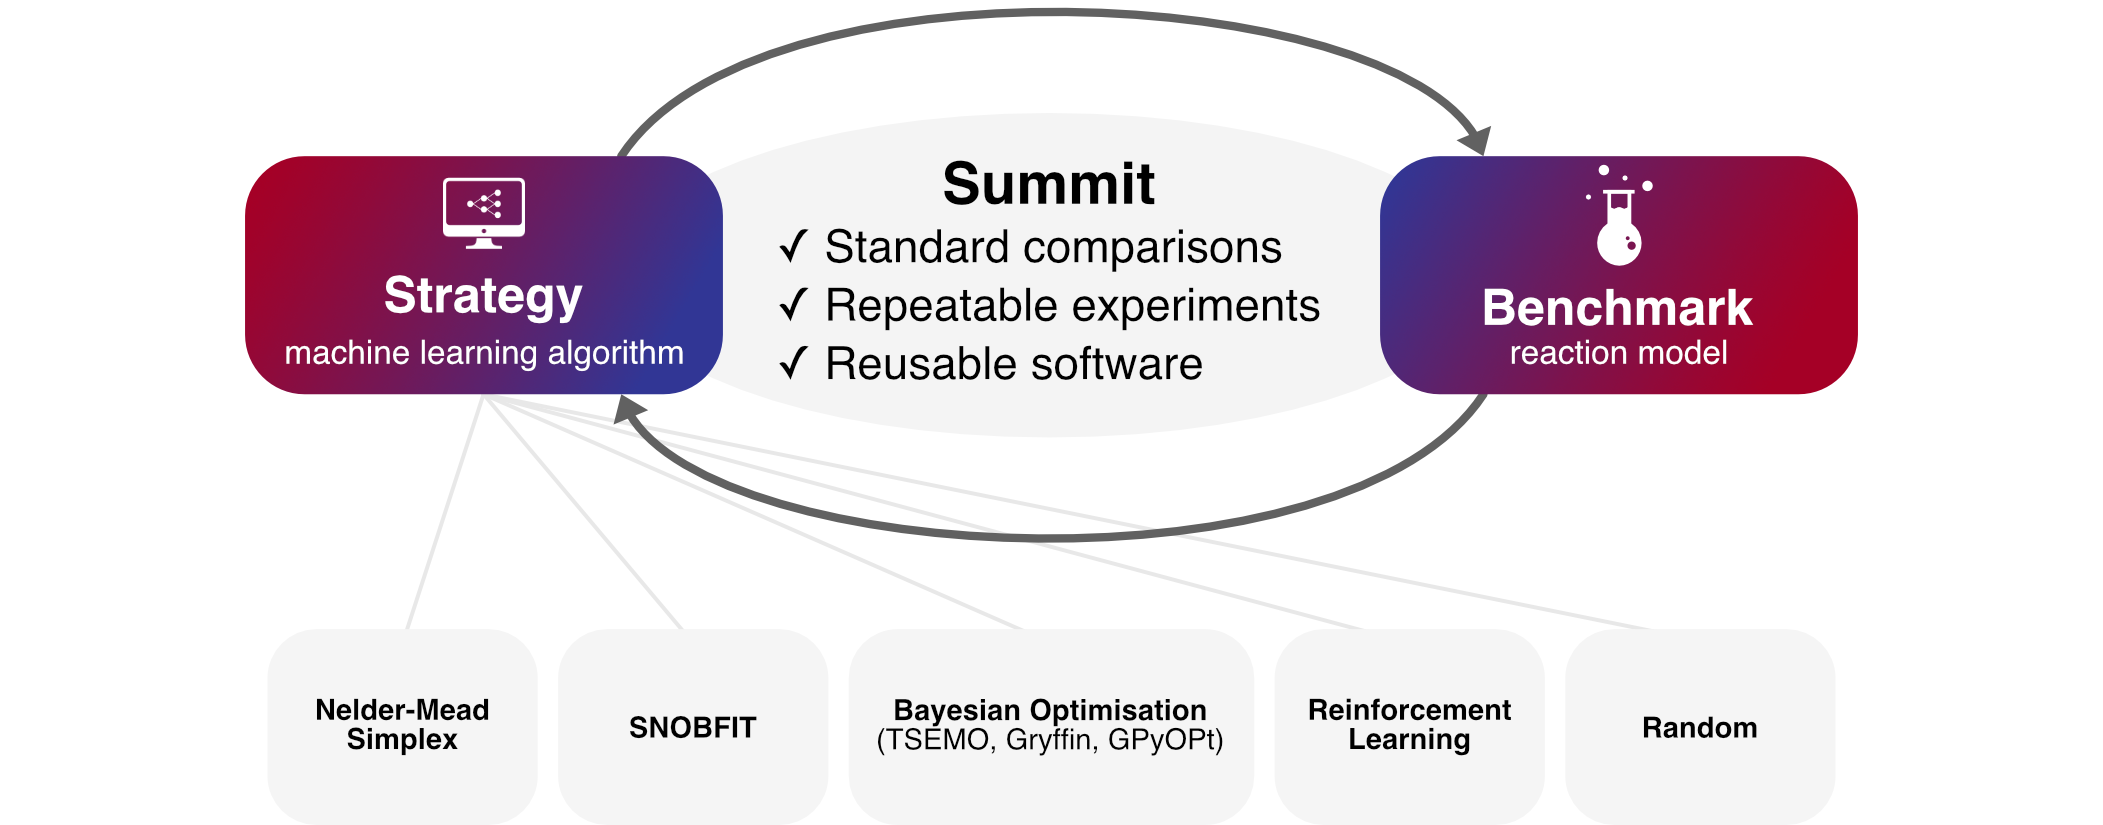
\includegraphics[width=\textwidth]{gfx/Chapter03/overview.png}
    \caption{Overview of the approach used by Summit. Strategies are machine learning algorithms or baselines. Benchmarks are models of reactions that simulate physical experiments. Strategies and benchmarks are used together in an iterative approach to find optimal reaction conditions. This software framework enables standard comparisons of strategies on different repeatable benchmarks without the need for expensive experiments. Furthermore, the same framework can be applied confidently to real experimental case studies.}
    \label{fig:overview}
\end{figure}

\section{Background}

\subsection{Self-optimisation}

Self-optimisation is a modern approach to automating the discovery of optimal reaction conditions for chemical processes, which does not require the determination of mechanistic models. Self-optimisation proceeds through iterative cycles of automated reaction execution, quantification, and algorithmic condition selection to efficiently identify optimal reaction conditions to maximize process metrics (yield, selectivity, etc.). Although self-optimisation was initially applied to tuning analytical instruments as early as the 1970s \cite{Routh1977}. Krishnadasan et al. \cite{Krishnadasan2007} first introduced the concept of self-optimisation of chemical reactions in 2007, which led to further adoption by many other research groups in the following years. Krishnadasan focused on the synthesis of CdSe quantum dots, but subsequent works have applied self-optimisation to a wide range of synthetic organic reactions \cite{McMullen2010a, McMullen2011, Bourne2011, Moore2012, christensen2021, Reizman2016b, Fitzpatrick2016,Echtermeyer2017}.

Self-optimisation is often conducted using automated reactors that can independently execute reactions at a specified set of reaction conditions. Automated analytical instruments then quantify the individual components of a reaction mixture, followed by an algorithmic suggestion of new reaction conditions based on previous data to improve key reaction outcomes. Self-optimisation research can therefore often be divided into three subsections that map directly on to these three key aspects: development of automated reactors, development of automated analytical methods and development of optimisation algorithms. One or more of these developments are typically reported in individual works in the literature. These ideas are shown conceptually in Figure \ref{fig:optimisation-cycle}.  In the following, I focus on optimisation algorithms, but I discuss in detail automated reactors and analytical methods in our review \cite{Taylor2023a}.

Chemical reactions can be viewed as mathematical functions that receive reaction conditions as input values and output reaction outcomes (e.g. product yield, selectivity etc.) \cite{Clayton2019}. This functional view of chemical reactions makes it clear why optimisation algorithms, which find the optimal values of mathematical functions, can be used to optimize chemical processes. optimisation algorithms iteratively evaluate the output of the function at different input values until a maximum or, if desired, a minimum, is reached. In the case of chemical processes, these iterative evaluations correspond with intelligently suggested experiments to execute in the laboratory until a set of reaction conditions are achieved that give the optimal desired output.

\begin{figure}
    \centering
    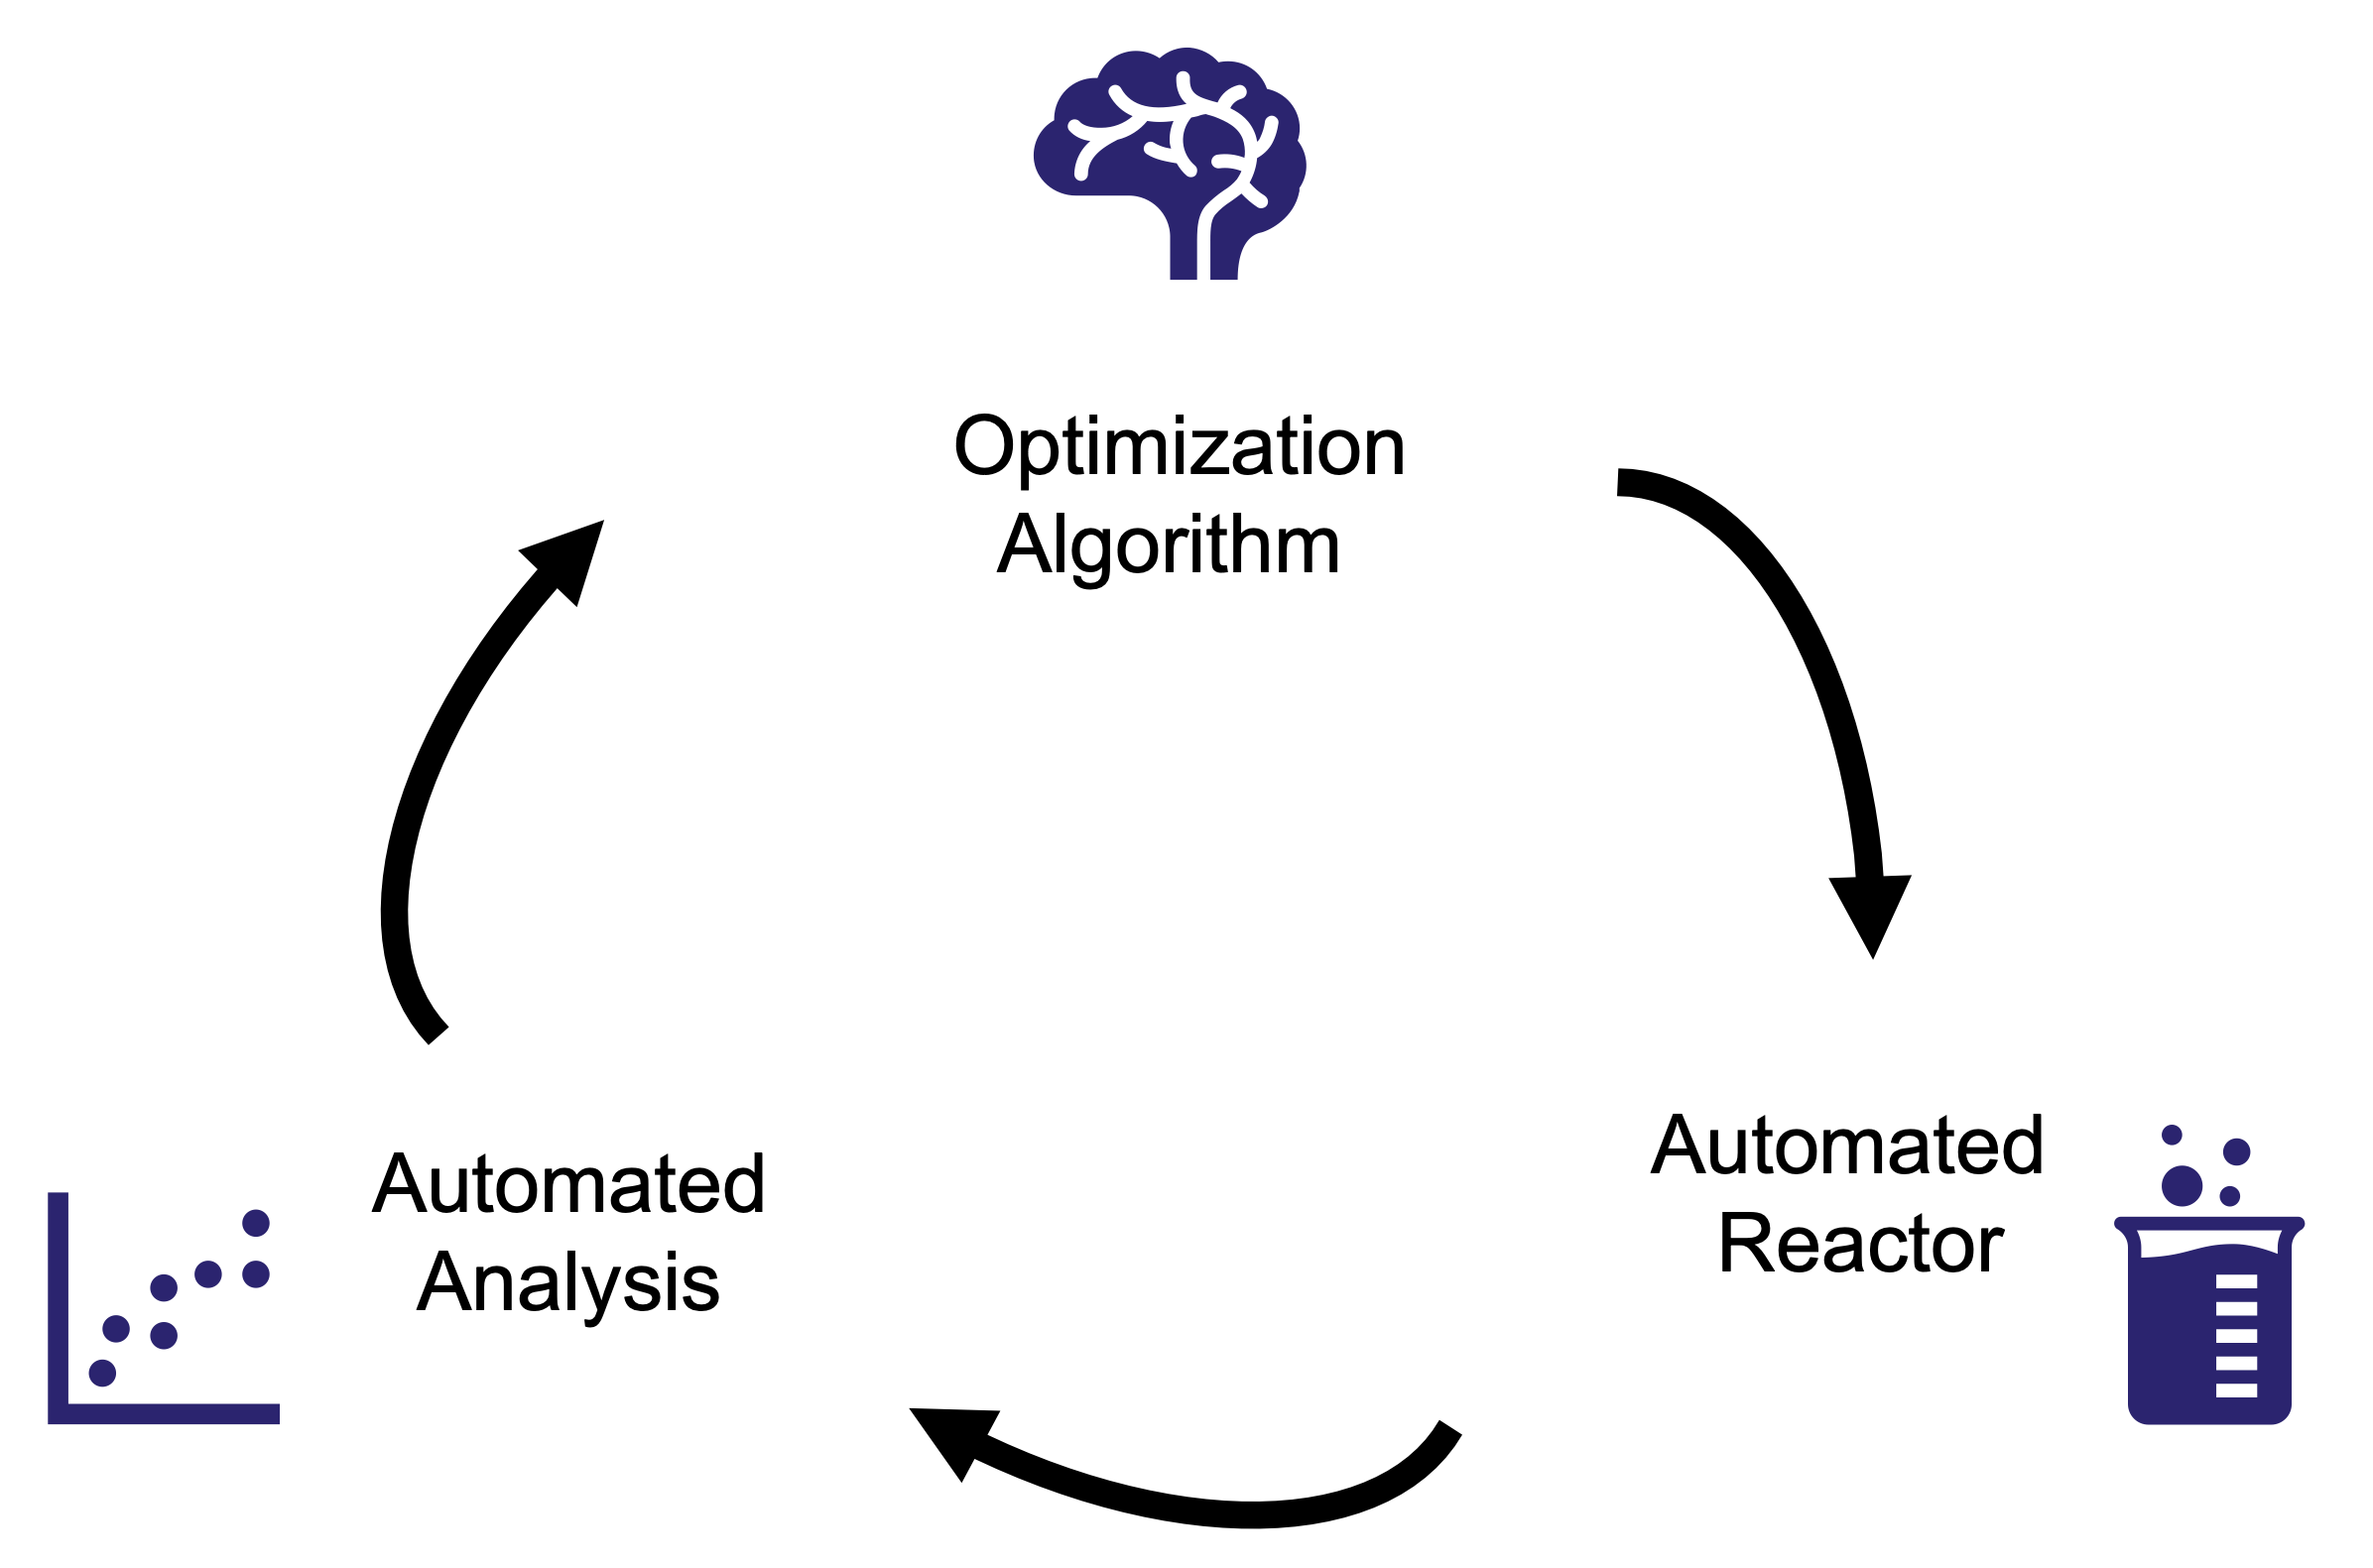
\includegraphics[width=0.9\textwidth]{gfx/Chapter03/self-optimization-cycle.png}
    \caption{The three parts of a self-optimizing reactor are: an automated reactor system, an analytical method and an optimisation algorithm.}
    \label{fig:optimisation-cycle}
\end{figure}

\subsection{Local vs Global optimisation}
The two main classes of optimisation algorithms are local and global optimisation algorithms. Local optimisation algorithms are designed to find the optimal values of a function closest to an initial guess. Therefore, if there is one optimal value, local optimisation algorithms will likely find it, but if there are multiple optima, the success of a local optimisation function is highly dependent on the initial guess. Example chemical applications of local optimisation algorithms include the steepest descent algorithm, which chooses reaction conditions based on the most favorable gradient (direction) in design space to explore \cite{McMullen2010a}, and the simplex algorithm, which explores design space based on geometric transformations to exploit perceived favorable areas \cite{Routh1977, Bourne2011}. The challenge with local optimisation algorithms is their dependence on the reaction conditions used to initialize the algorithm; if there are multiple regions of chemical space with local optima, the algorithm could potentially fail to find the best overall reaction conditions for the transformation, as illustrated in Figure \ref{fig:local-optimisation}.

\begin{figure}
    \centering
    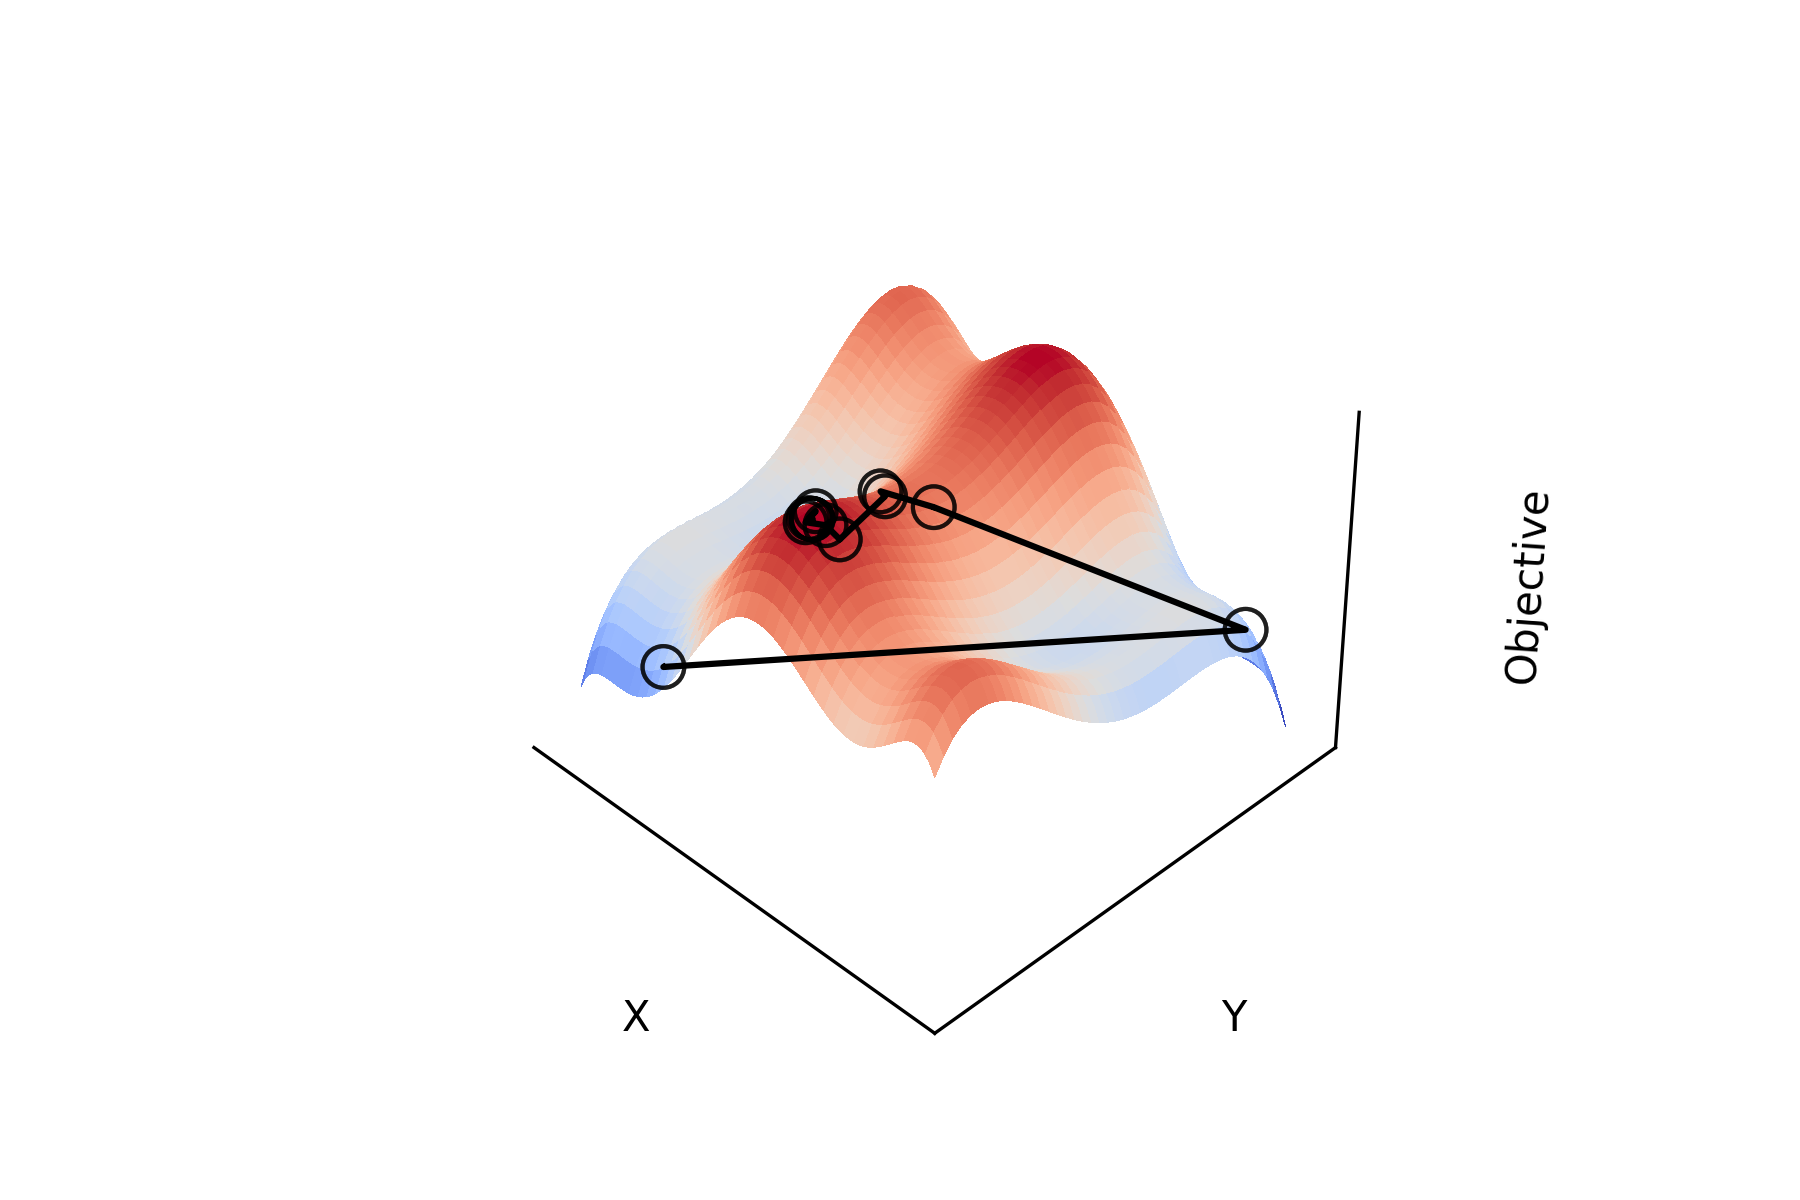
\includegraphics[width=0.8\textwidth]{gfx/Chapter03/local_optimzation.png}
    \caption{An illustration of a local optimisation algorithm failing to find the global maximum of a function with multiple local optima. X and Y are hypothetical experimental variables (e.g. temperature, reaction time) and the objective is the value that must be maximized (e.g. yield). Unfilled circles are function evaluations (i.e. experiments). Red indicates local maxima function value, while blue indicates local minima.}
    \label{fig:local-optimisation}
\end{figure}
 
Global optimisation algorithms can identify the best value of a function independent of the initial guess but may require more experiments to obtain this global optimum. Krishnadasan and several other researchers were the first to apply global optimisation to self-optimisation \cite{Holmes2016b, Krishnadasan2007, McMullen2010a}. They used the Stable Noisy Branch and Fit (SNOBFIT), which splits the domain into several hypercubes and balances the search across these subdivisions. \cite{Huyer2008}. Early work in the field found that SNOBFIT was effective at optimising difficult reaction problems \cite{McMullen2010a}.

More recently, researchers have demonstrated the effectiveness of Bayesian optimisation (BO) algorithms for reaction optimization \cite{Schweidtmann2018, Amar2019, Hase2020, Shields2021, Manson2021}. For example, in work contemporary to Summit, Shields et al. showed that BO was efficient at optimizing both \textit{in silico} benchmarks and experimental case studies \cite{Shields2021}. Overall, Bayesian optimisation offers a principled and efficient way to apply global optimisation to chemical reactions and is discussed in more detail in Chapter \ref{ch:background}.

\subsection{Categorical Variables}
Each of the aforementioned algorithms only utilize continuous input variables (e.g. temperature, concentration, residence time), but chemistry problems often have categorical variables also (e.g. solvent, ligand etc.). To address this algorithmic limitation, the Jensen group used a branch-and-fit algorithm that eliminates possible values for categorical variables (e.g. particular solvents, ligands etc.) that resulted in low yield or high turn-over number \cite{Reizman2016a, Baumgartner2018}. This approach is less efficient when compared to newer algorithms due to the need to fit a separate model for each categorical variable instead of developing one global model.

Alternatively, it is possible to use optimisation algorithms that inherently work with categorical variables. In two recent studies, Bayesian optimisation algorithms were adapted to automatically learn the relationship between categorical variables from experimental data \cite{Manson2021, Hase2021}. These algorithms tended to perform slightly better in finding optimal reaction conditions than the aforementioned strategies that could not learn a relationship between categorical variables and may be a large research area of interest in future. Note that categorical variables can be explored by quantifying them with various ‘continuous variable’ molecular parametrizations, though this is usually not effective in the limit of small data \cite{Pomberger2023}.

\subsection{Multi-objective optimisation}
Optimisation problems in chemistry often involve trade-offs between multiple competing objectives, such as balancing high process yields with low costs, so optimisation algorithms need to be able to consider and weight these objectives to find optimal solutions. The approaches used in the early literature on self-optimisation place important objectives as constraints (e.g., requiring a minimum yield) \cite{Reizman2015b, Reizman2016a, Reizman2016b, Baumgartner2018} or used weighted functions of multiple objectives \cite{Krishnadasan2007, Fitzpatrick2016, Hase2018b}. These approaches result in a single optimum point, when it is expected that multiple optimum points would be available representing different trade-offs.

A better approach is to use multi-objective optimisation algorithms. These algorithms aim to find the Pareto front or set of solutions for which an improvement in one objective would cause a worsening of another. Figure \ref{fig:schweidtmann_example} shows an example of the multi-objective Bayesian optimisation algorithm TSEMO \cite{Bradford2018} applied to a N-benzylation reaction \cite{Schweidtmann2018}. The flow rate of $\alpha$-methylbenzylamine 1.1, ratio of benzyl bromide 1.2 to 1.1, solvent flow rate and temperature were modified to maximize production of 1.3, while minimizing formation of 1.4. After 20 experiments designed by Latin hypercube sampling (LHS) \cite{McKay1979}, a balanced random sampling technique, TSEMO quickly identified 58 further experimental conditions on or near the Pareto front. The Pareto front indicated that a 60 $kg m^{-3} h^{-1}$ increase in space-time yield (STY) would correspond with approximate 10 \% increase in impurity yield, and a scientist could then choose how to balance this trade-off.

\begin{figure}
    \centering
    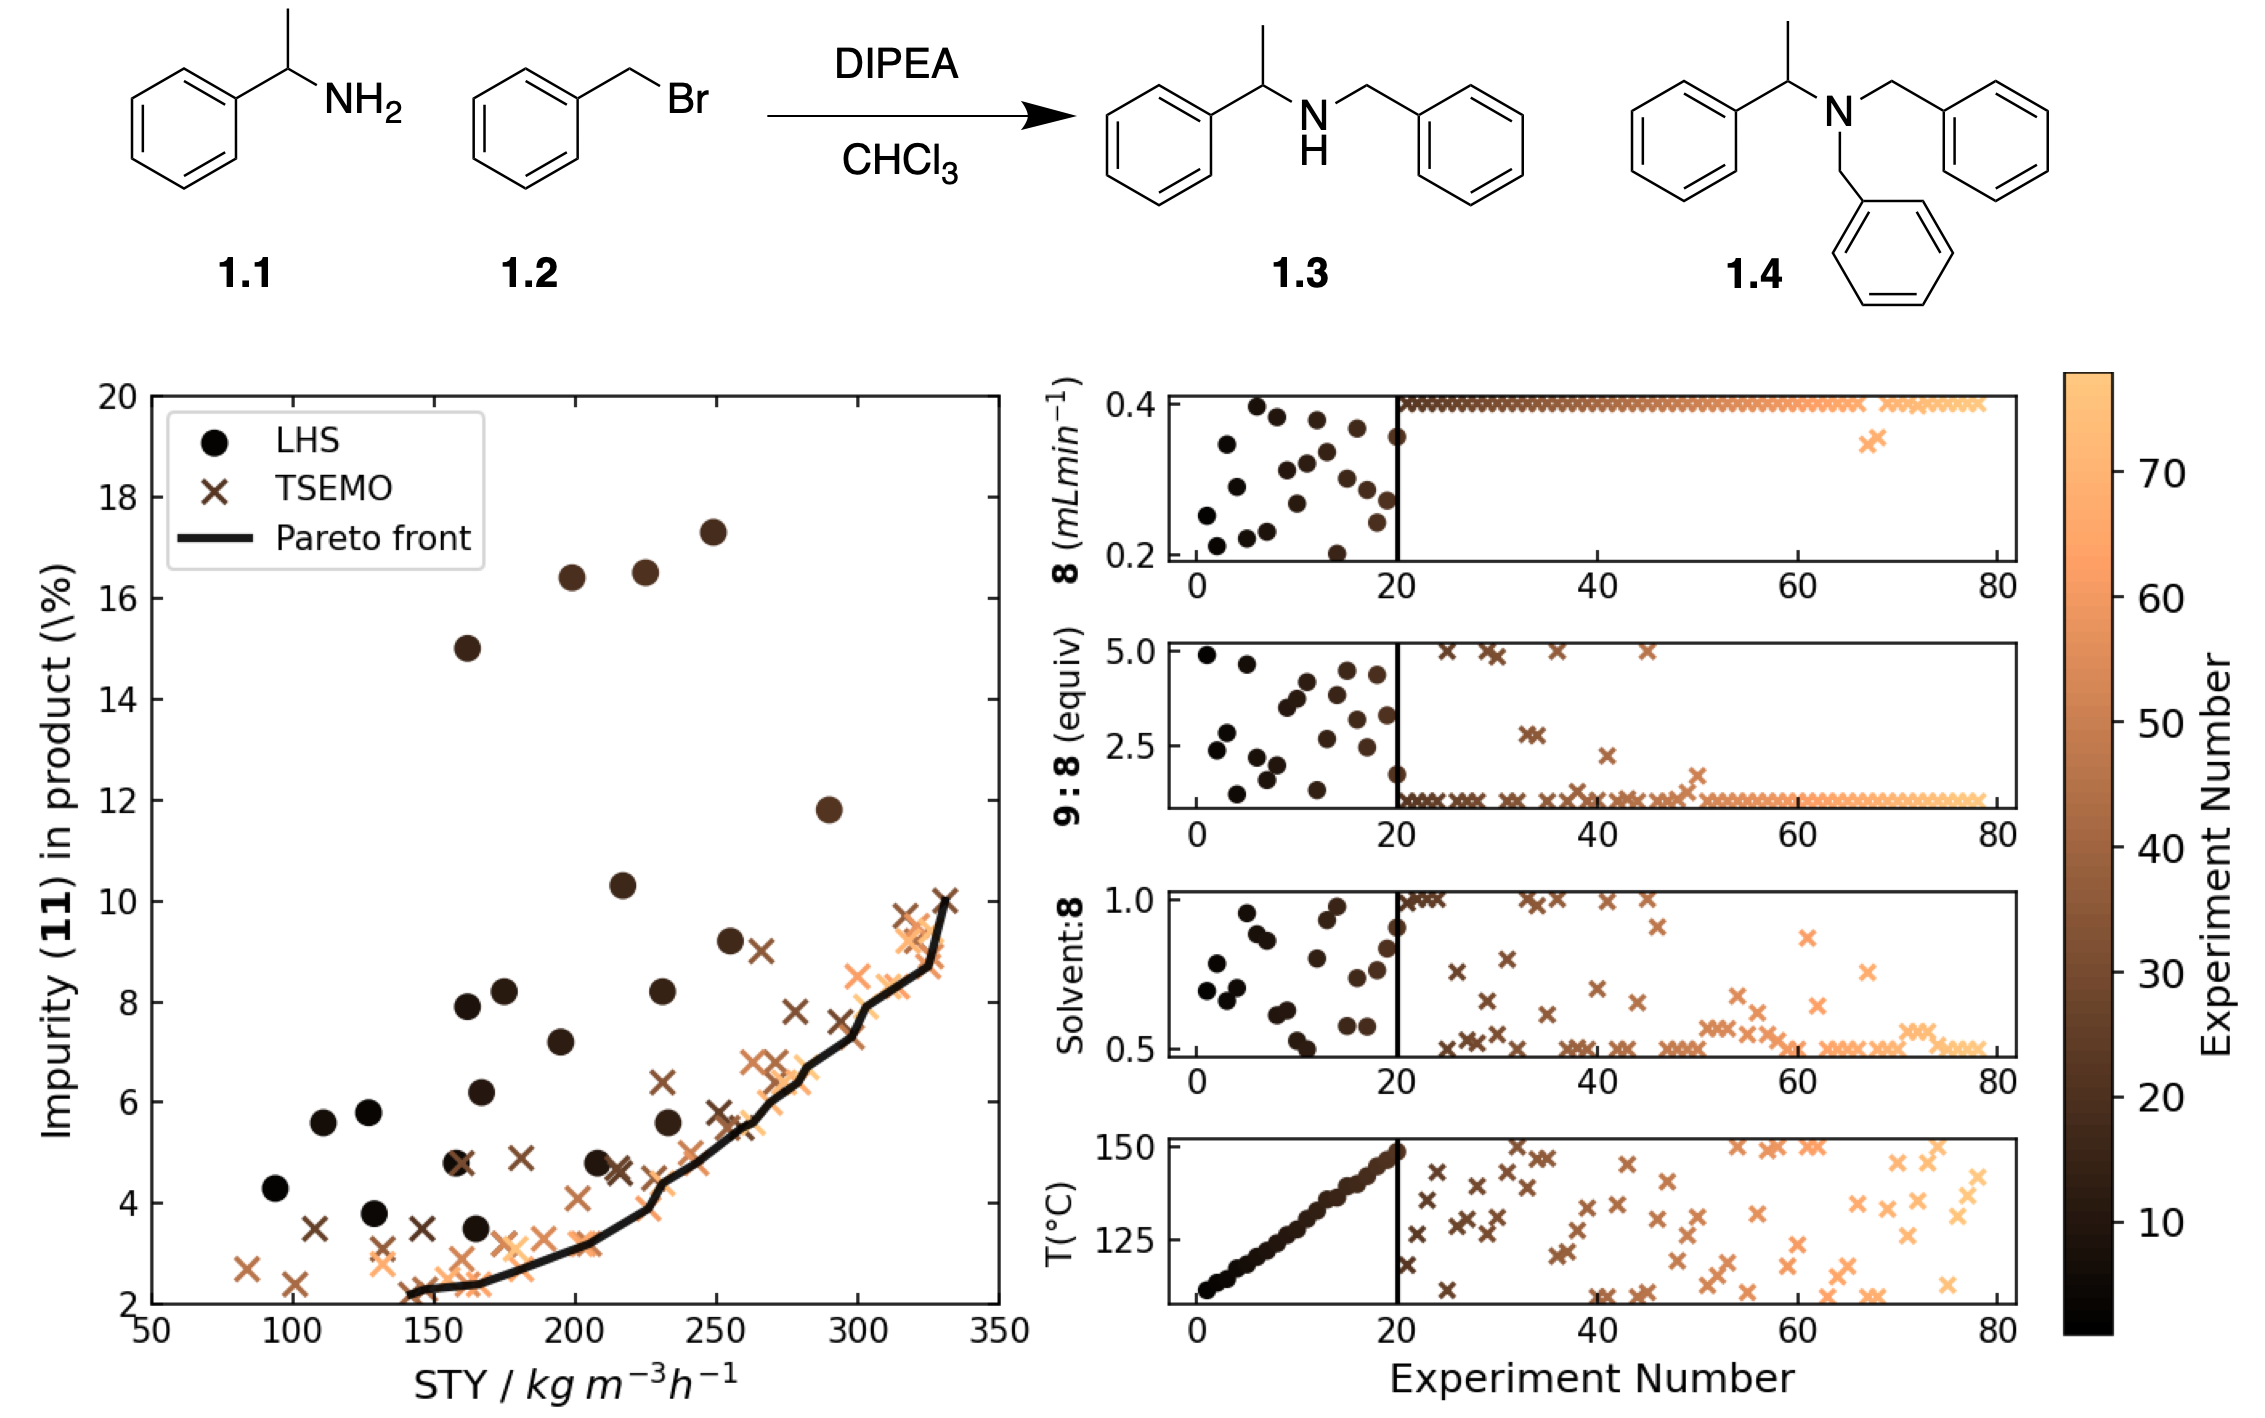
\includegraphics[width=\textwidth]{gfx/Chapter03/schweidtmann_thesis.png}
    \caption{Multi-objective self-optimisation of the N-benzylation of N-benzylation of $\alpha$-methylbenzylamine \textbf{1.1} with benzyl bromide \textbf{1.2} \cite{Schweidtmann2018}. TSEMO \cite{Bradford2018} was used to maximize space time yield of the desired 2° amine \textbf{1.3} and minimize production of the percent impurity of 3° amine \textbf{1.4}. After 20 experiments designed by Latin hypercube sampling (LHS) \cite{McKay1979}, TSEMO quickly identified experiments on or near the Pareto front.}
    \label{fig:schweidtmann_example}
\end{figure}

% \subsection{Transfer Learning for Reaction optimisation}

% Self-optimisation has shown promise in the automated optimisation of single reactions, but there is a wealth of reaction data available that current algorithms are unable to utilize. Very recent work has used transfer learning techniques to accelerate optimisation by leveraging data from similar reaction optimisation campaigns, but this has mainly been demonstrated \textit{in silico } \cite{Hickman2022}, with one active learning example from Pomberger et al. with the focus of pH adjustment \cite{Pomberger2023}. In this work, I use the Summit to develop the optimal settings for multi-task Bayesian optimisation (MTBO) and then, in collaboration with an experimentalists, demonstrate its effectiveness in the lab.

% MTBO was originally developed to speed up hyperparameter tuning of machine learning models (e.g., choosing learning rates and batch sizes to maximize model accuracy) \cite{Swersky2013}. Using only the hyperparameters and resulting model accuracy scores of a previously trained machine learning model (which I call Task A),  MTBO decreased by up to 50\% the the number of experiments needed to find optimal hyperparameters for a new machine learning model (which I call Task B).  The data from Task A helped the model better predict Task B, even with only a few experiments for Task B.

% Multi-task Bayesian optimisation (MTBO) uses a multi-task probabilistic model inside a BO framework.  Swersky et al. were the first to demonstrate that multi-task BO can be effectively used to accelerate BO for hyperparameter tuning of machine learning models \cite{Swersky2013}. They demonstrated that using the results of hyperparameter tuning on one dataset could assist in tuning another with multi-task GPs. In many cases, multi-task BO could achieve 40-50\% improvements in the test accuracy of models with significantly feIr training runs.  

% One of the challenges faced in applying MTBO to big data uses cases has been its lack of scalability. This in mainly due to the $O(n^3)$ cost of using GPs with exact inference. Several different approaches have been taken to solving this problem including training a vanilla neural network on the tasks and feeding the output to a Bayesian linear regression model \cite{Perrone2018} and using the auxiliary tasks to create a learned feature representation in a compressed space \cite{Hakhamaneshi2021}. These methods have retained the performance of multi-task BO while minimizing the computational cost of its deployment. However, in our case, all datasets have less than 1000 points and in many cases, less than 100. This makes multi-task GPs with exact inference more tractable.

% Another direction has been to apply the machinery of multi-task GPs to multifidelity BO, which aims to leverage data from a cheap but less accurate data source to help with optimizing a more expensive function. This technique has been applied in a wide range of scenarios including parameter estimation of physics models using data from multiple experiments and simulations;\cite{Perdikaris2016} optimizing battery electrode structure using data from both cheap and expensive multitscale differential equation models (Pan 2017), and optimizing composition of alloys using a mix of DFT fidelities (Tran 2020). I foresee that, given these results, our approach will be able to be extended to combine data from simulations and experiments to rapidly optimize processes.


\section{Methods}

\subsection{Summit}
Summit is the first python package dedicated to reaction optimisation. Summit is available as open-source software on \textbf{\href{https://github.com/sustainable-processes/summit}{Github}}.  Summit was designed with the principles of simplicity and  flexibility in mind. I used python due its prevalence in data science and the availability of machine learning packages such as Tensorflow \cite{tensorflow2015} and PyTorch \cite{Paszke2019}. Summit has two main components: benchmarks and strategies.
    
Benchmarks are simulations of reactions. I propose two approaches to developing benchmarks in Summit. The first is to use mechanistic models that include reaction kinetics and potentially other phenomena such as mass transport. These models are typically differential equations that can be integrated to find reaction yield and selectivity \cite{Reizman2015b, Baumgartner2018}. In Summit, these equations are easily integrated using numerical integration software available in packages like SciPy, \cite{2020SciPy-NMeth} and a standard interface saves researchers the time of re-implementing common functionality. 

Alternatively, when a mechanistic model is not available, it is possible to create a data-driven benchmark. Data-driven benchmarks are machine learning models trained on experimental data to predict yield or other reaction performance metrics given reaction conditions \cite{Hase2020a}.  If data is available in the form of a CSV file, this can be achieved in Summit using as little as two lines of code. I include a base class called \textit{Experiment} which is inherited by benchmarks. One noteworthy functionality is the \textit{ExperimentalEmulator} which creates a benchmark from data by training a machine learning algorithm to predict reaction outcomes given reaction conditions. The overall process involves specifying the decision variables and objectives; importing experimental data from a CSV file and using one line of code to train the model. Strategies contain the logic for machine learning algorithms. Each strategy has a \textit{suggest\_experiments} method, which takes in a dataset with any previous experimental data and generates conditions for a new set of experiments.  Since Summit is written according to object oriented methodologies, new strategies can easily inherit and override the functionality of existing strategies.

In Figure \ref{fig:code_example}, I demonstrate how these components can be combined to run a closed-loop optimisation of the $S_NAr$ benchmark in Summit (described in Section \ref{subsec:mechanistic_benchmarks}). In the first line of code, the benchmarks is instantiated, and line two, one of the strategies, TSEMO, is instantiated by passing in the domain from teh benchmark. Domains describe the decision variables and objectives of the benchmark. Finally, I pass the strategy and benchmark to the constructor for \textit{Runner}, which will run closed loop optimisation automatically and report back the results. In the subsequent sections, I describe the benchmarks and strategies used in this chapter.

\begin{figure}
    \centering
    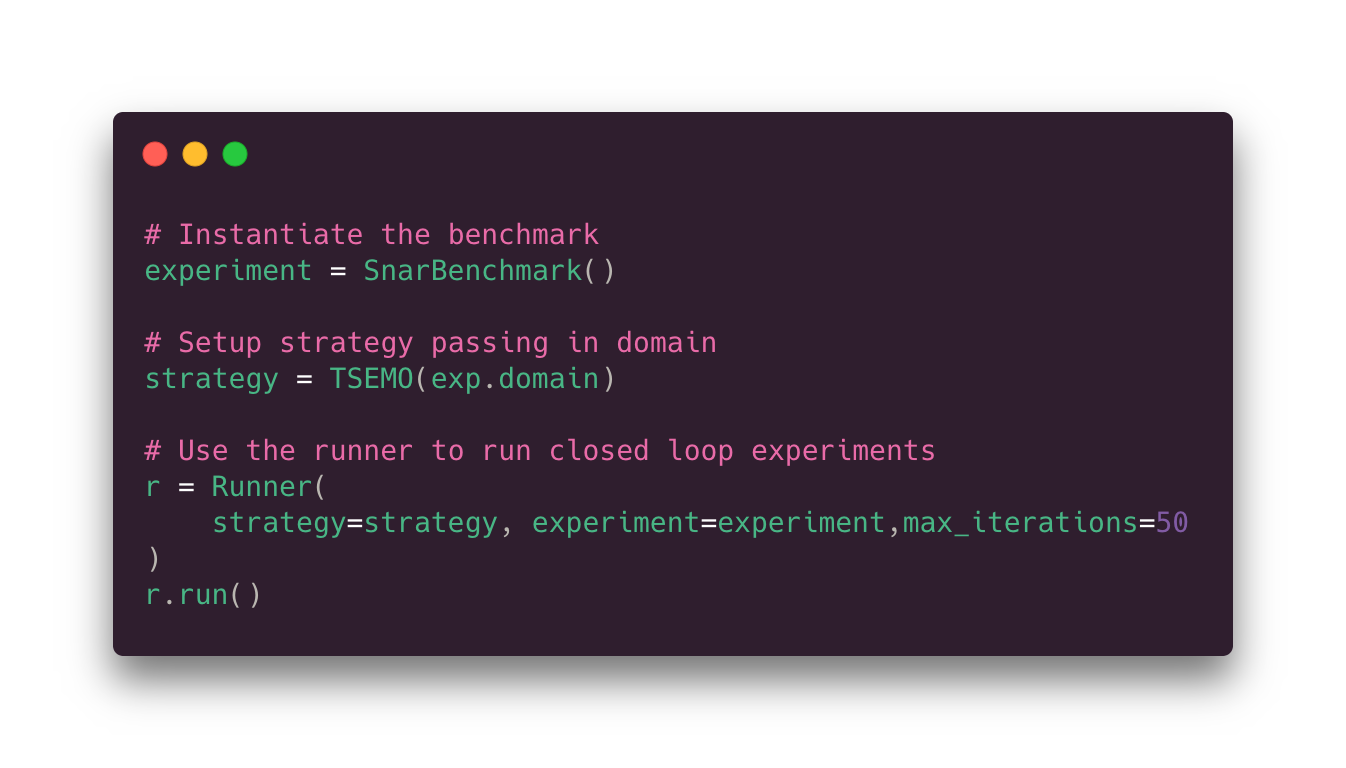
\includegraphics[width=\textwidth]{gfx/Chapter03/paraiso.png}
    \caption{Example code for creating a benchmarking study using Summit.}
    \label{fig:code_example}
\end{figure}



\subsection{Benchmarks}

I chose as benchmarks reactions which are well-understood or could be modeled using machine learning. Therefore, it is possible to focus the studies on this chapter on comparing the quality of various optimisation strategies. The subsequent chapter contains experimental validation on a challenging case study.

\subsubsection{Mechanistic Benchmarks}\label{subsec:mechanistic_benchmarks}

The $S_NAr$ benchmark is a reaction between 2,4-difluoronitrobenzene \textbf{3.5} and pyrrolidine \textbf{3.6} to afford the desired products \textbf{3.7} with \textbf{3.8} and \textbf{3.9} as undesired side-products \cite{Hone2017}. Here, the aim is to optimise the reaction in a virtual self-optimising flow setup, as shown in Figure \ref{fig:snar}a. Formally, the optimisation problem can be stated as simultaneously maximising space time yield ($STY$) and minimizing the E-factor ($E$), which is a measure of environmental impact of a reaction  \cite{Sheldon2017}. The decision variables (i.e,. the reaction conditions) are the temperature (40-120 $^{\circ}$C), residence time (0.5-2 minutes), equivalents of \textbf{3.6} (1.0-5.0) and concentration of difluoronitrobenzene (0.1-0.5M). As noted in Equation \ref{snar_formal}, this is achieved by adjusting the residence time $\tau$, inlet concentration of \textbf{3.5} $C_{3.5,i}$, equivalents of pyrrolidine $n_{3.6}$, and reactor temperature, $T$.
\begin{equation}
	\label{snar_formal}
	\begin{gathered}
		\min_{X}{(-STY, E)} \\
		\text{where}\;\; X = [\tau,C_{3.5,i},n_{3.6}, T]
	\end{gathered}
\end{equation}


\begin{figure}
    \centering
    \subfloat[]{
        \centering
        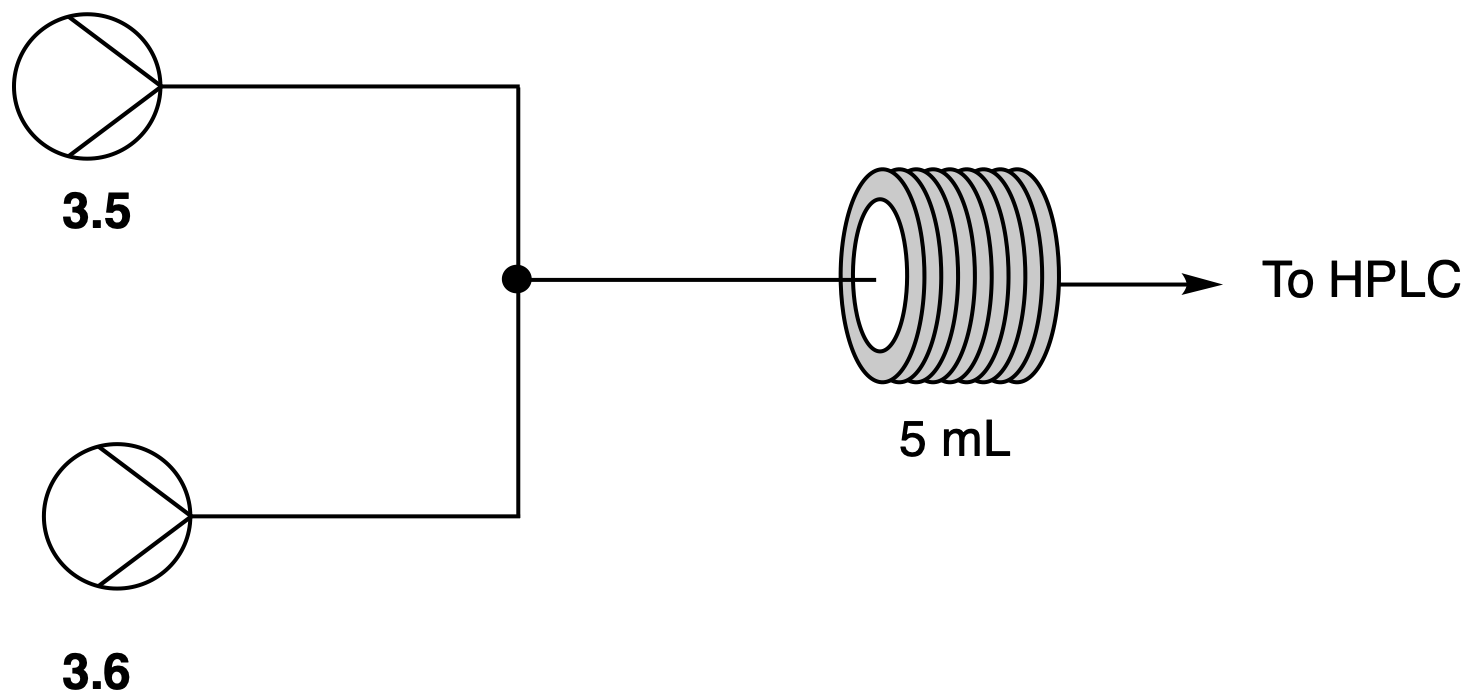
\includegraphics[width=0.5\textwidth]{gfx/Chapter03/flow_snar}
        % \subcaption{}
    }
    \subfloat[]{
        \centering
        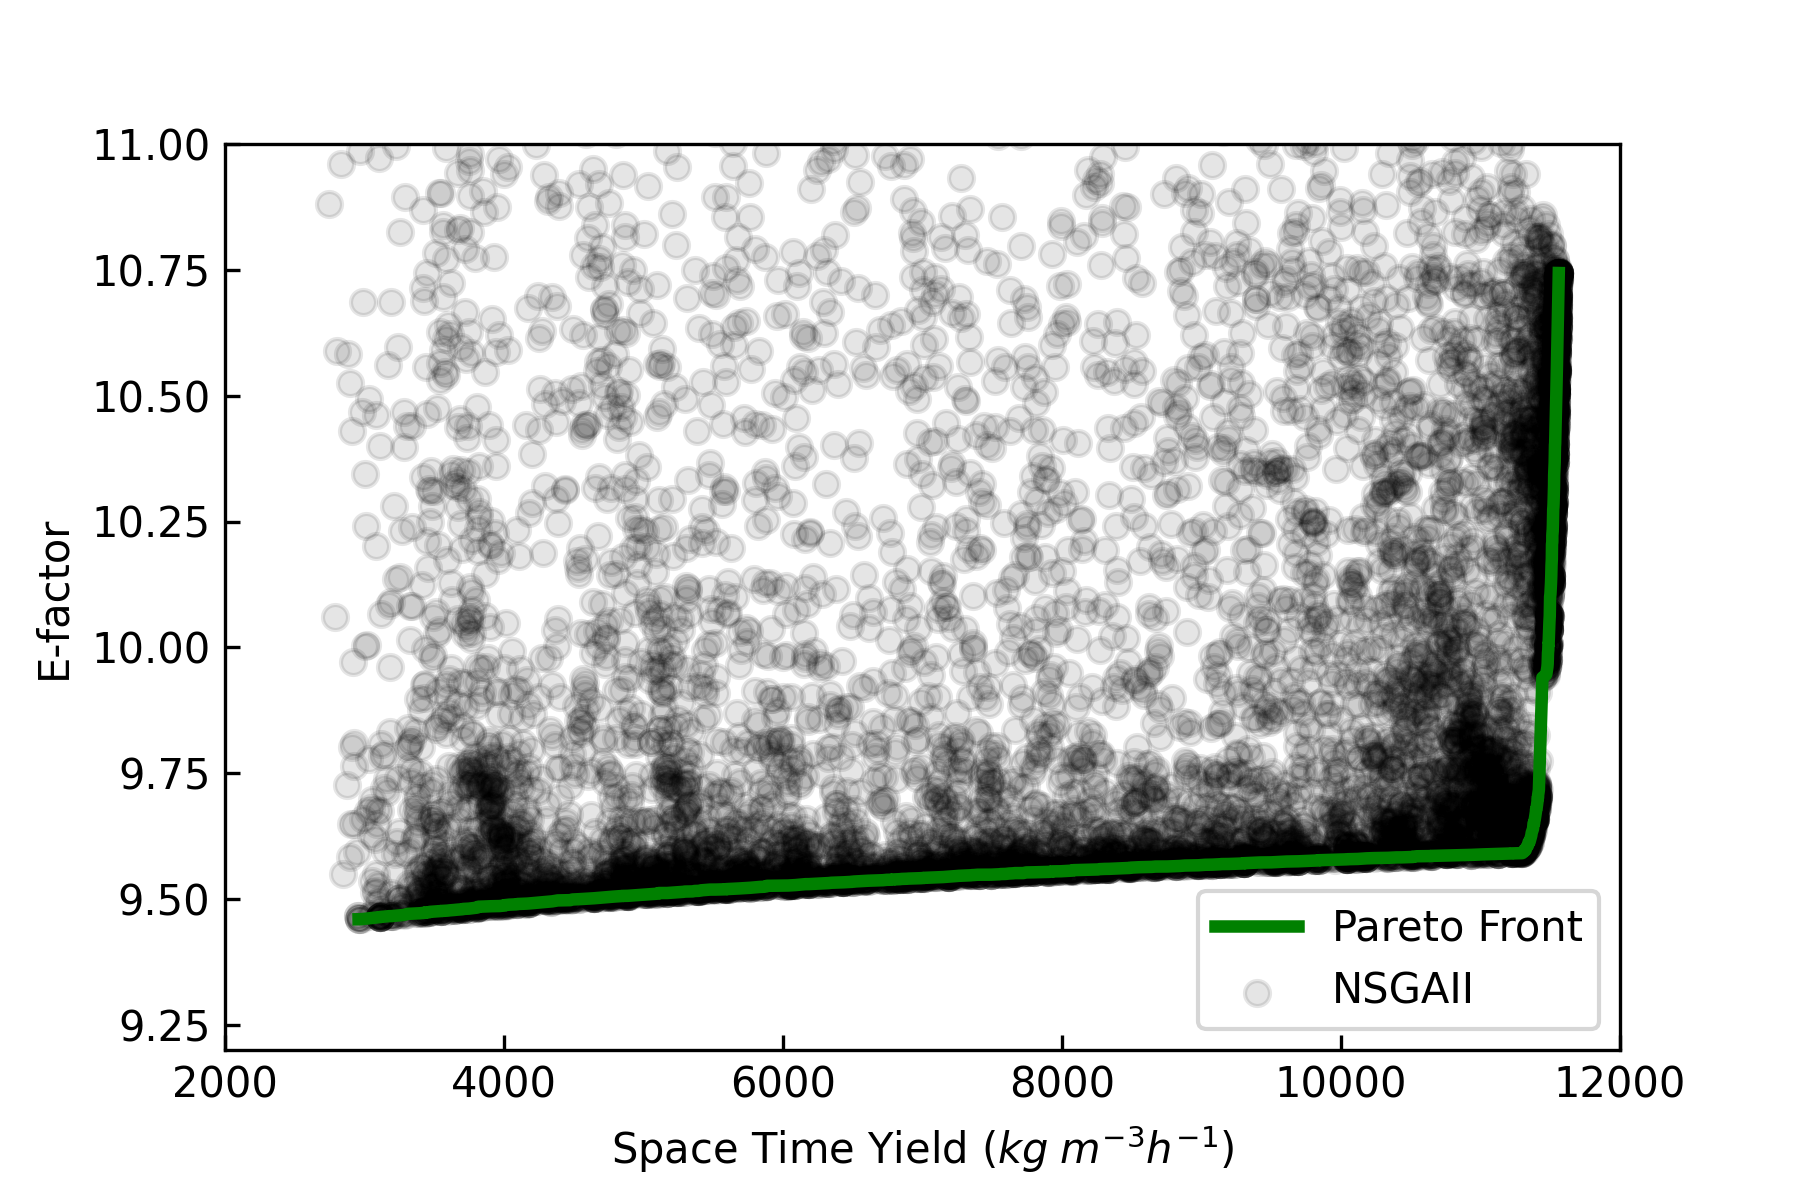
\includegraphics[width=0.5\textwidth]{gfx/Chapter03/pareto_front_snar.png}
        % \subcaption{}
    }
    \caption{(a) Schematic of the virtual flow chemistry reactor used in the benchmark. (b) optimisation landscape of S$_N$Ar benchmark as determined by running NSGA-II for 100 generations with a population size of 100.}
    \label{fig:snar}

\end{figure}

I use hypervolume as a performance metric, which measures the volume in any number dimensions dominated by the Pareto front \cite{Emmerich2016}. To calculate hypervolume, a reference is needed. I use the Nadir point as a reference (i.e., negative of the edges of the Pareto front), which is estimated by running the NSGA-II optimisation algorithm \cite{Deb2002} on the S$_N$Ar benchmark for 100 generations with a population size of 100. As shown in \ref{fig:snar}b, the Pareto front  extends over a wide range of space time yields (2500-12 000) and a narrow range of E-factors (9.5-10.75). The Nadir point is estimated as (-2957, 10.7), given that the STY is negated to account for hypervolume assuming minimisation.

\begin{figure}
    \centering
    
\includegraphics[width=\textwidth]{gfx/Chapter03/snar_benchmark_scheme_thesis.png}
    \caption{Scheme showing the reaction being optimized for $S_NAr$ benchmark. This is a four dimensional optimisation of a  S\textsubscript{N}Ar reaction between difluoronitrobenzene (\textbf{3.5}) and pyrrollidine (\textbf{3.6}) \cite{Hone2017}.}
    \label{fig:snar_benchmark}
\end{figure}

I now show the equations used to calculate the objective values for given a set of conditions. Space time yield ($STY$) is defined as the mass of 3.7 leaving the reactor per residence time ($\tau$), and E-factor ($E$) is defined as the ratio of mass of waste to mass of product:

\begin{equation}
    \label{sty}
	STY = \frac{M_{3.7} C_{3.7}}{\tau}
\end{equation}
\begin{equation}
    \label{e_factor}
	\begin{split}
	 E & = \frac{m_{waste}}{m_{product}} \\ 
	   & = \frac{Q_{tot}\rho_{eth} + \sum_{n=1, i \neq 3}^5 M_nC_nQ_{tot}}{M_{3.7}C_{3.7}Q_{tot}}		
	\end{split}
\end{equation}
where $M_n$ is the molar weight of species $n$; $Q_{eth}$ and $\rho_{eth}$ are the volumetric flowrate the density of ethanol respectively; and $Q_{tot}$ is the total volumetric flowrate. The volume of the reactor is assumed to be 5 mL. The inlet concentration of \textbf{3.6} is calculated:
\begin{equation}
    C_{3.6,i} = n_{3.6} C_{3.5,i}
\end{equation}
$n_{3.6}$ is the equivalents of pyrrolidine. Since the total flowrate $Q_{tot}$ is $\frac{V}{\tau}$, then flowrates of the pumps are calculated as:
\begin{equation}
    Q_1 = \frac{C_{3.5,i}}{C_{1,0}}Q_{tot}
\end{equation}
\begin{equation}
    Q_2 = \frac{C_{3.6,i}}{C_{2,0}}Q_{tot}
\end{equation}
where $C_{1,0}=1 M$ and $C_{2,0}=2 M$ are the reservoir concentrations of \textbf{3.5} and \textbf{3.6  } respectively. To calculate the outlet concentrations of the products, the standard equation for a constant density plug flow reactor is used:
\begin{equation}
	\label{pfr}
	d\tau = \frac{dC_n}{- r_n}
\end{equation}
where $C_n$ and $r_n$ are the concentration and reaction rate of species $n$, respectively. Hone et al. determined the reaction rates to be first order with kinetic constants $k_l$ (see Table \ref{table:snar_parameters}) in each species \cite{Hone2017}:
\begin{equation}
    \label{equation:r_1}
	r_{1} = -(k_1+k_2)C_{3.5}C_{3.6}	
\end{equation}
\begin{equation}
	r_2 = -(k_1+k_2)C_{3.5}C_{3.6}-k_3C_{3.6}C_{3.7}-k_4C_{3.6}C_{3.8}
\end{equation}
\begin{equation}
	r_3 = k_1C_{3.5}C_{3.6}-k_3C_{3.6}C_{3.7}
\end{equation}
\begin{equation}
	r_4 = k_1C_{3.5}C_{3.6}-k_4C_{3.6}C_{3.8}
	\label{equation:r_4}
\end{equation}
\begin{equation}
	\label{last_snar_rxn_rate}
	r_5 = k_3C_{3.6}C_{3.7} + k_4C_{3.6}C_{3.8}
\end{equation}

\begin{table}[tb]
  \centering
  \caption{Kinetic parameters used for the $S_NAr$ benchmark based on work by Hone et al \cite{Hone2017}.}
  \begin{tabular}{ccc}
    &$k_{l,ref} \; (10^{-2} \text{mol}^{-1} \text{dm}^3 \text{s}^{-1})$ & $E_a$ (kJ $\text{mol}^{-1}$) \\
    \hline
    $k_{1,ref}$ & 57.9 & 33.3  \\
    $k_{2,ref}$ & 2.70 & 35.3  \\
    $k_{3,ref}$ & 0.865 & 38.9 \\
    $k_{4,ref}$ & 1.63 & 44.8 \\
  \end{tabular}
  
  \label{table:snar_parameters}
\end{table}

The kinetic constants $k_l$ for each reaction are calculated using the Arrhenius equation:
\begin{equation}
	k_l = k_{l, ref} \exp\Biggl[-\frac{E_{a,l}}{R}\biggl(\frac{1}{T}-\frac{1}{T_{ref}}\biggr)\Biggr]
\end{equation}
where $k_{l, \\ref}$ is the constant at the reference temperature $T_{ref}$ of $90^{\circ}$C and $E_{a,l}$ is the activation energy. The five differential equations described by Equation \ref{pfr} and Equations \ref{equation:r_1}-\ref{equation:r_4} are integrated over the residence time to find the final concentrations given the inlet concentrations of each species $C_{n,i}$. These concentrations are then supplied to Equations \ref{sty} and \ref{e_factor} to calculate the space time yield and E-factor.

% \ref{fig:snar_pareto_fronts} shows the estimated Pareto fronts for the best run of each unique combination of strategy, transform, and number of initial experiments. The best run is determined by the terminal hypervolume.  The reference for the hypervolume calculations is (0, 1). TSEMO finds the best combinations of high space-time-yield and E-factor. Note that for the Custom multi-objective transform, the following objective was minimised: $-STY/1000+E/100$. \ref{tab:snar_benchmark_results} gives the complete results.

% \begin{figure}[p]
%     \centering
%     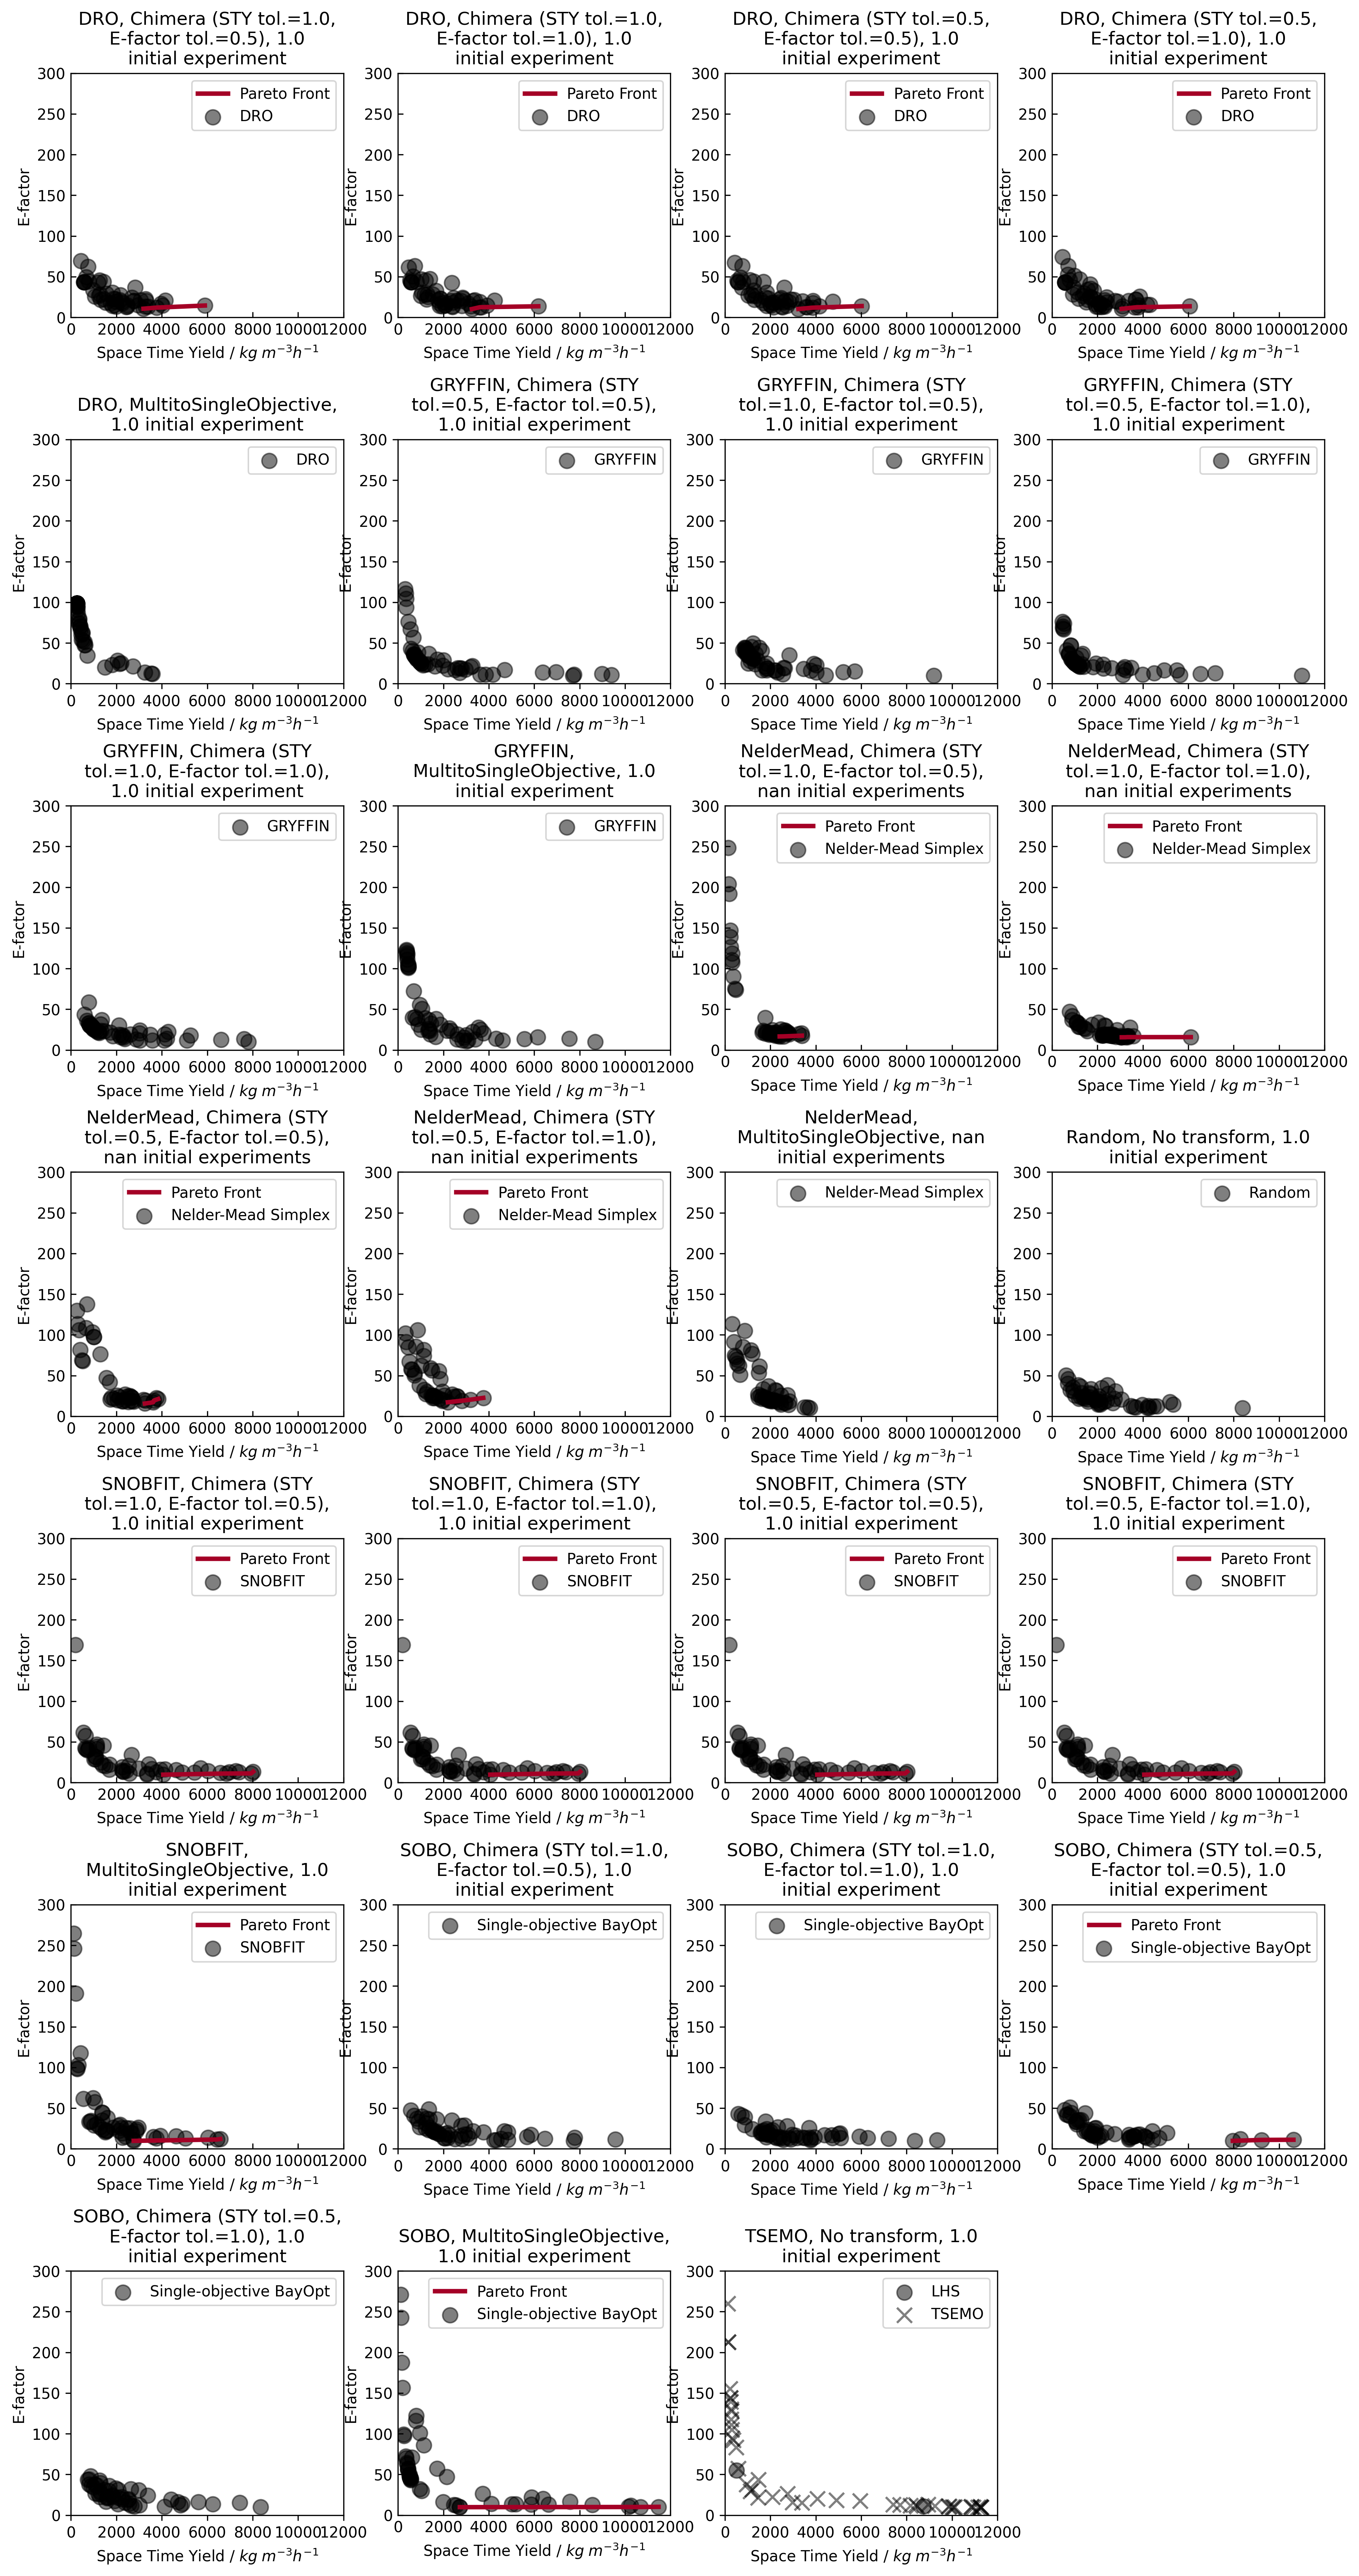
\includegraphics[height=0.8\textheight]{figures/snar_pareto_fronts.png}
%     \caption{Pareto fronts for the best run (by terminal hypervolume) of each unique combination of strategy, transform, and number of initial experiments for the SnAr benchmark.}
%     \label{fig:snar_pareto_fronts}
% \end{figure}

 
\subsubsection{Data-driven benchmarks}

As shown in Figure \ref{fig:benchmarks_cn_summit}b, the second benchmark is the optimisation of a Pd-catalysed C-N cross coupling reaction. The C-N benchmark represents a Pd-catalyzed cross coupling between aryl triflate and aniline \cite{Baumgartner2019}. This is a five dimensional optimisation of temperature, residence time, base equivalents, catalyst and base. The catalyst choices are t-BuXPhos, t-BuBrettPhos, AlPhos. The bases are TEA, TMG, BTMG, and DBU. The categorical variables (catalyst and base) contain descriptors that are pre-calculated using COSMOQuick computational fluid thermodynamics program \cite{Loschen2012}. The descriptor are the $\sigma$-moments, which are interpretable and general descriptors for any molecule \cite{Zissimos2002}. We use the first two $\sigma$-moments which correspond with area and polarizability respectively.

The yield is determined using a Bayesian Neural Network (BNN) that is trained on the experimental data from Baumgartner et al. \cite{Baumgartner2019}. The BNN is implemented in PyTorch \cite{Paszke2019} using the BLITZ library \cite{Esposito2020}. The total dataset contains 96 experiments, where 86 experiment are used for training of the model and 10 experiments are held out as a test set for evaluation of the model. The model is trained using 10-fold cross validation. A mean absolute error of 0.08 is achieved on the test set.


\begin{figure}[p]
    \centering
    
\includegraphics[width=0.9\textwidth]{gfx/Chapter03/c_n_benchmarks_thesis_2.png}
    \caption{Optimisation of a C-N cross coupling between aniline (\textbf{1.11}) and aryl triflate (\textbf{1.12}).\cite{Baumgartner2019} The strategies must select one of three Buchwald catalysts and one of four organic bases for each experiment. Additionally, strategies must select the temperature, residence time, and base equivalents. The objectives are to maximise yield and minimise cost.}
    \label{fig:benchmarks_cn_summit}
\end{figure}


% \begin{figure}[p]
%     \centering
%     
\includegraphics[width=0.9\textwidth]{gfx/Chapter03/suzuki_benchmarks_thesis.png}
%     \caption{Reaction schemes for the Suzuki cross coupling benchmarks used in this chapter. The data for training the benchmarks are taken from Baumgartner et al. \cite{Baumgartner2018} and \cite{Reizman2016b}. Optimizing these reactions requires tuning continuous variables catalyst loading, reaction time and temperature as Ill as selecting from a library of Buchwald G3 catalysts \cite{Bruno2013}.}
%     \label{fig:benchmarks_suzuki}
% \end{figure}


\subsection{Strategies}

\subsubsection{Bayesian optimisation}

In addition to the standard single objective Bayesian optimisation (BO) described in Chapter \ref{ch:background}, this chapter uses to other BO strategies: TSEMO and Gryffin.

TSEMO is an abbreviation for Thompson sampling efficient multi-objective optimisation \cite{Bradford2018}. As the name suggests, TSEMO is an adaptation of BO to multi-objective problems. TSEMO uses an independent GP for each objective. Instead of the Expected Improvement as an acquisition function, TSEMO maximizes the hypervolume improvement, which is a measure of the improvement of the Pareto front with an additional predicted point. Instead of using the posterior directly, TESMO samples a deterministic function using Random Fourier features. This enables use of an evolutionary multi-objective optimisation algorithm NSGA-II \cite{Deb2002} to create a list of potential candidate experiment which can then be ranked by maximum hypervolume improvement to choose one or more suggestions..

Gryffin is a BO approach concerning the challenge of categorical input variables in optimisation and was recently presented by H{\"{a}}se et al \cite{Hase2020a}. Gryffin offers to support the optimisation algorithm by including domain knowledge in the form of assigning descriptors to the possible values of the categorical input variables (categorical options). Since descriptors provide information about similarity or diversity of the categorical options, Gryffin utilizes this additional information by redefining the distance between the different categorical options depending on the their respective associated descriptor values. So, instead of using the frequently employed one-hot encoding of categorical options with similar distance between all options,  Gryffin defines the distance between categorical options to be the euclidean distance of the real-valued descriptors uniquely assigned to each option. In this way, a relationship of different categorical options is quantified and becomes measurable, providing additional knowledge to the optimisation algorithm. 

% Multi-task BO (MTBO) replaces the GP in Bayesian optimisation with a multi-task GP. I use the intrinsic model of coregionalization originally proposed by Bonilla et al. \cite{Bonilla2007}, which defines a multi-task kernel $k^{ICM}_{\theta}$ as the Kronecker product of standard GP kernel (the Matérn kernel in our case) and a task kernel $k^t_{\theta}$:
% \begin{equation}
%     k^{ICM}_{\theta}(x,x') = k^t_{\theta} \otimes  k_{\theta}(x,x')
% \end{equation}
% The task kernel $k^t_{\theta}$ is a $T \times T$ matrix of trainable parameters where $T$ is the number of tasks. These parameters represent the inter-task correlation.

\subsubsection{SNOBFIT}
SNOBFIT or Stable Noisy optimisation by Branch and Fit is a derivative-free optimisation algorithm  \cite{Huyer2008}.  After an initial SNOBFIT call with a randomized space-filling design, exploitation is realized by fitting local quadratic  models of the objective function for each point that has been evaluated. Then, SNOBFIT suggests new points by optimising these quadratic models. In addition to exploitation, points in unexplored regions of the problem domain are suggested. My collaborator Jan Rittig noticed that SNOBFIT sometimes suggests more experiments than requested by the user. This is most common if the number of experiments is low. I believe this could be caused by the exploratory part of SNOBFIT, but further investigation would be needed to make a conclusive determination.

 \subsubsection{Nelder-Mead Simplex}
The Nelder-Mead Simplex (NMS)\cite{Nelder1965} is a local optimisation algorithm.  NMS optimises an objective function using multi-dimensional polyhedra. For an optimisation problem with $n_{DoF}$ degrees of freedom, the NMS spans a polyhedra with $n_{DoF} + 1$ vertices within the feasible domain. Each vertex represents a set of conditions with the corresponding objective function value.  During the optimisation process, vertices with the worst objective function values are replaced iteratively by applying geometrical operations to the polyhedra: reflection, expansion, contraction, and shrinking. 

There are several limitations to NMS. First, a different number of experiments are requested in advance of each the distinct geometrical operation. Therefore, it is impossible to request a fixed number of experiments from NMS.  Second, since NMS only considers a local region of the problem domain, it can converge to local optima. 
\subsubsection{Reinforcement Learning}
Reinforcement learning agents learn to make optimal decisions given information about a problem \cite{sutton2018reinforcement}. These agents consist of a policy, which takes in a state (e.g., previously tried reaction conditions and corresponding yields) and suggests an action (e.g., a new set of reaction conditions). The optimality of an action or a set of actions is quantified through a reward. Reinforcement learning is discussed in more detail in Chapter \ref{ch:rl_tuning}. Zhou et al. built the bridge from RL to optimizing chemical reactions: an algorithm that (decision-maker) sequentially suggests experiments to carry out (actions) resulting in the highest yield (reward) \cite{Zhou2017}.

Thereby, they proposed the Deep Reaction optimiser (DRO), a recurrent neural network architecture with a RL-motivated loss function that is proportional to the yield obtained from each experiment suggested and carried out. It was assumed that the response surfaces for chemical reactions are continuous and can be approximated by Gaussian processes (GPs). Thus, the DRO was pretrained on GPs in order to simulate optimising the response surfaces of chemical reactions. These pretrained models were then inferred to yield optimisation of actual chemical reactions.

\subsection{Multi-objective Transforms}

Some strategies are not compatible with multi-objective domains by default. As shown in Figure \ref{fig:transforms}a, multi-objective transforms aim to convert multi-objective optimisation problems into single objective optimisation problems. This makes a wider range of strategies amenable to multi-objective problems. These transforms are often called achievement scalarisation functions (ASFs).

\begin{figure}
    \subfloat[]{
        \centering
        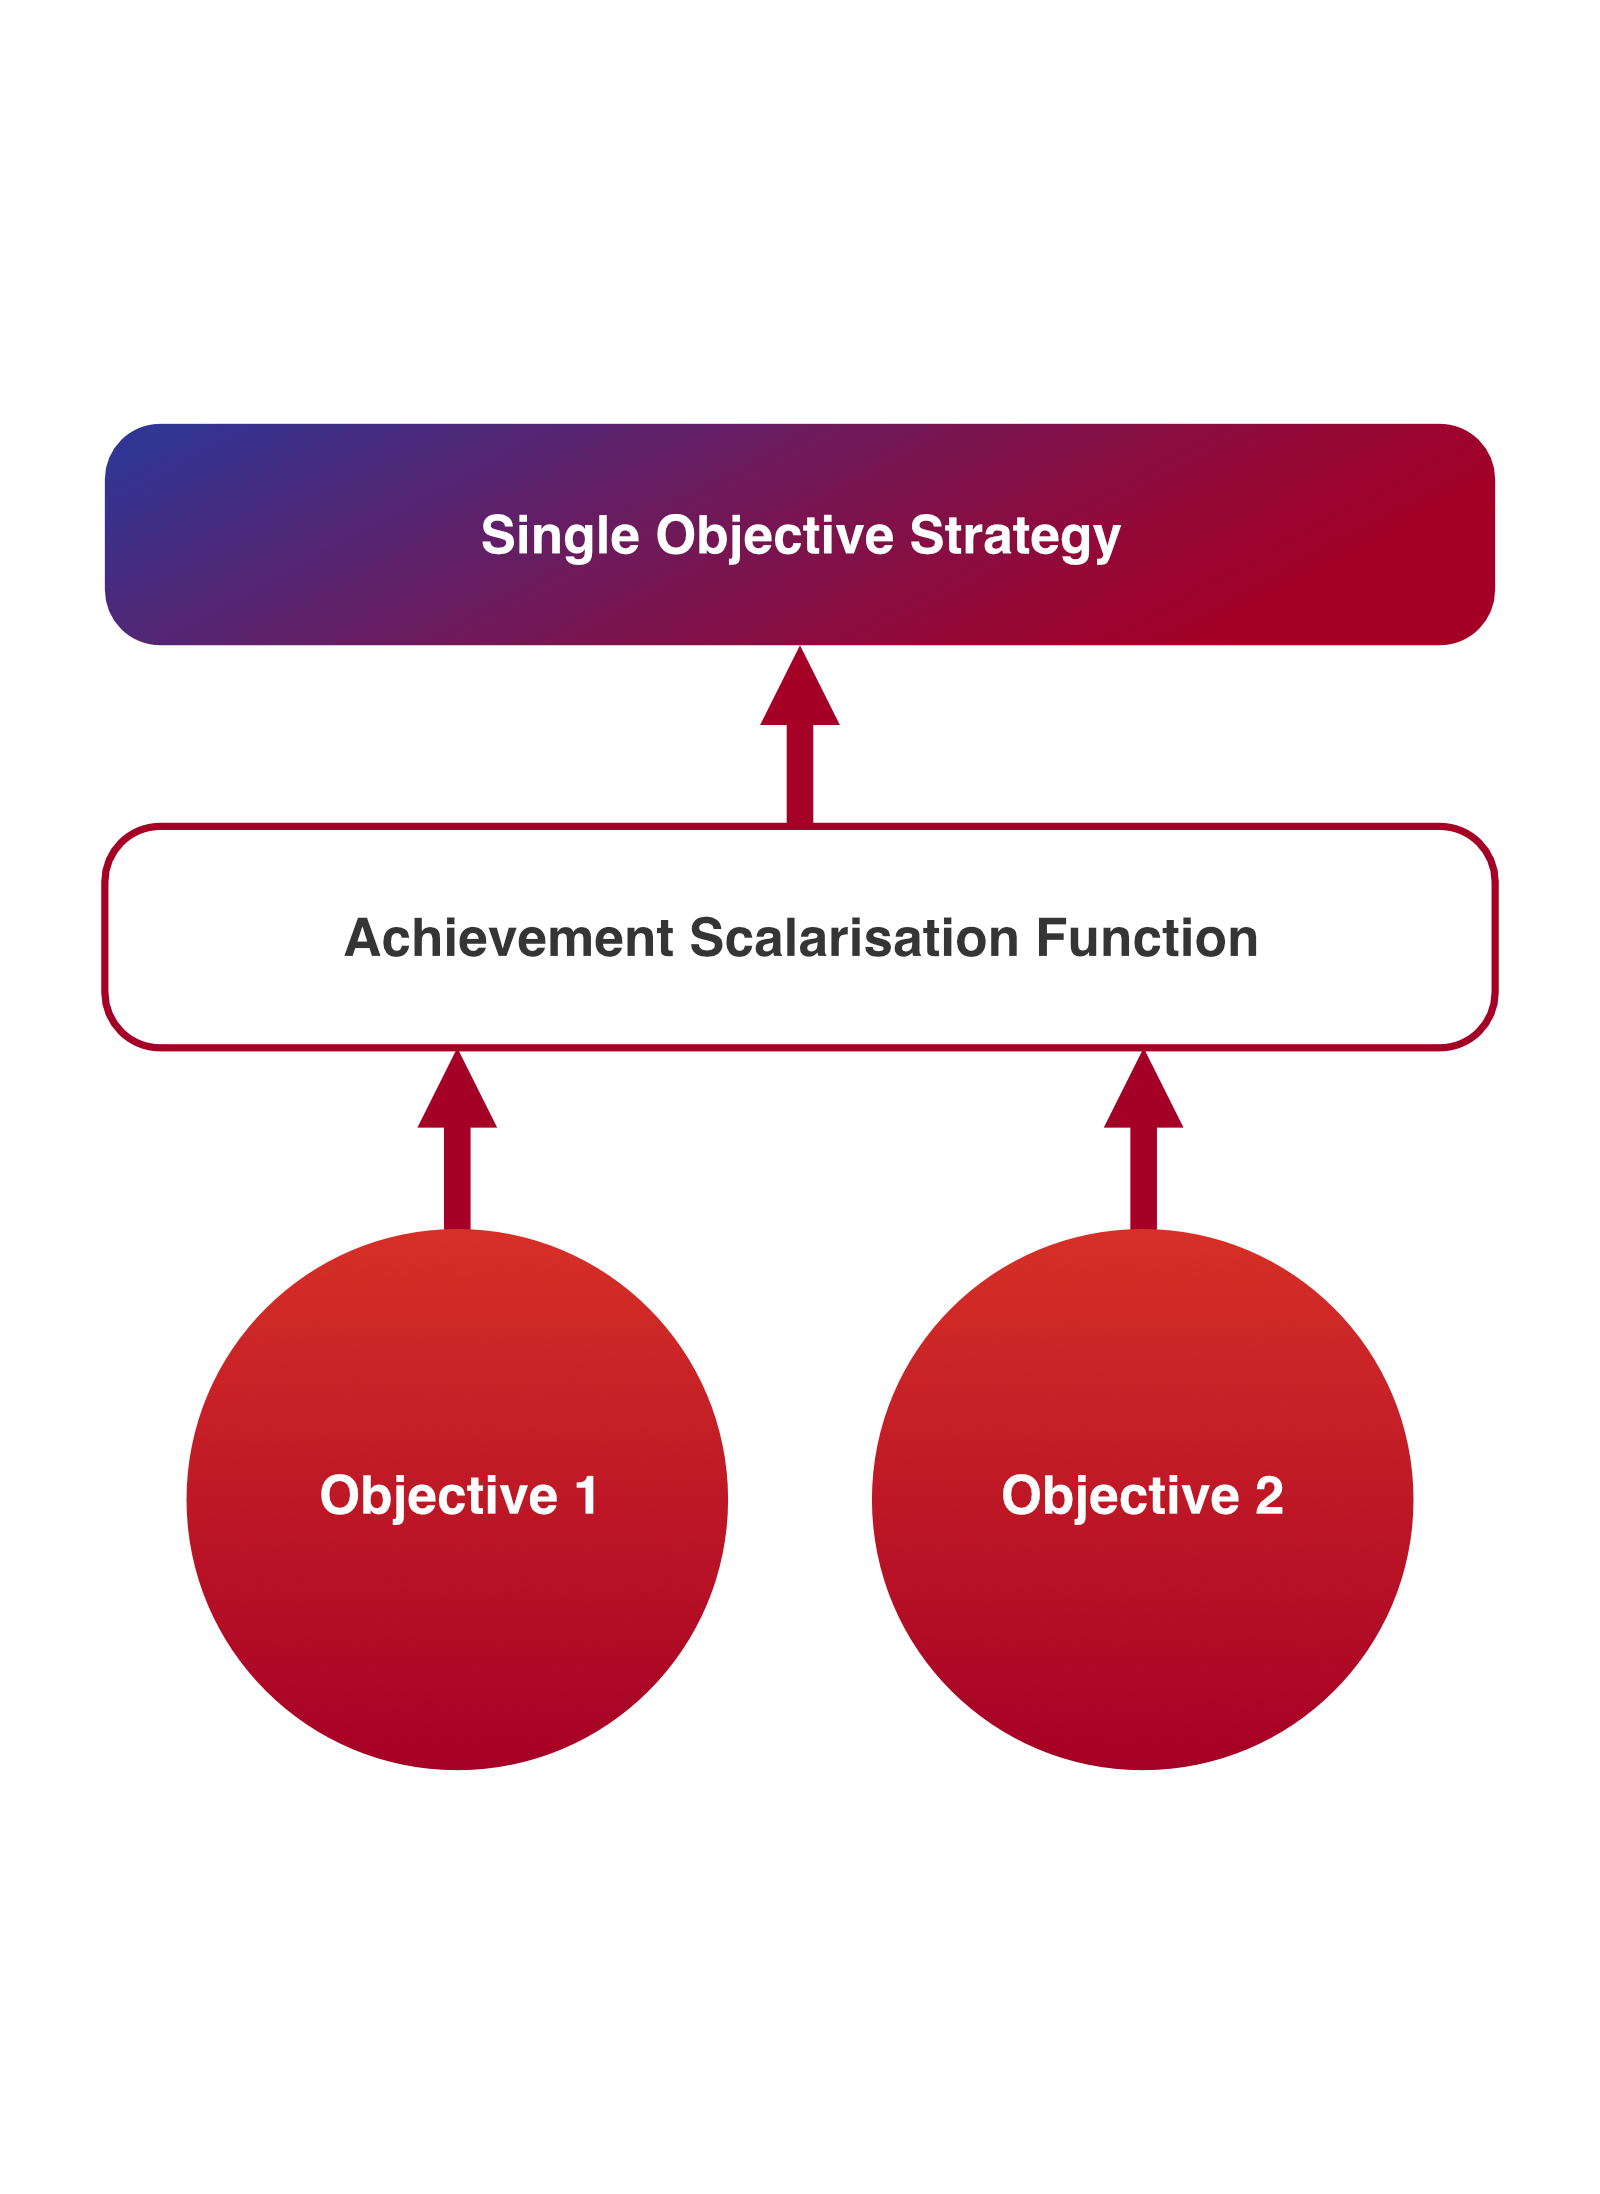
\includegraphics[width=0.5\linewidth]{gfx/Chapter03/custom_asf.png}
        
    }
    \subfloat[]{
        \centering
        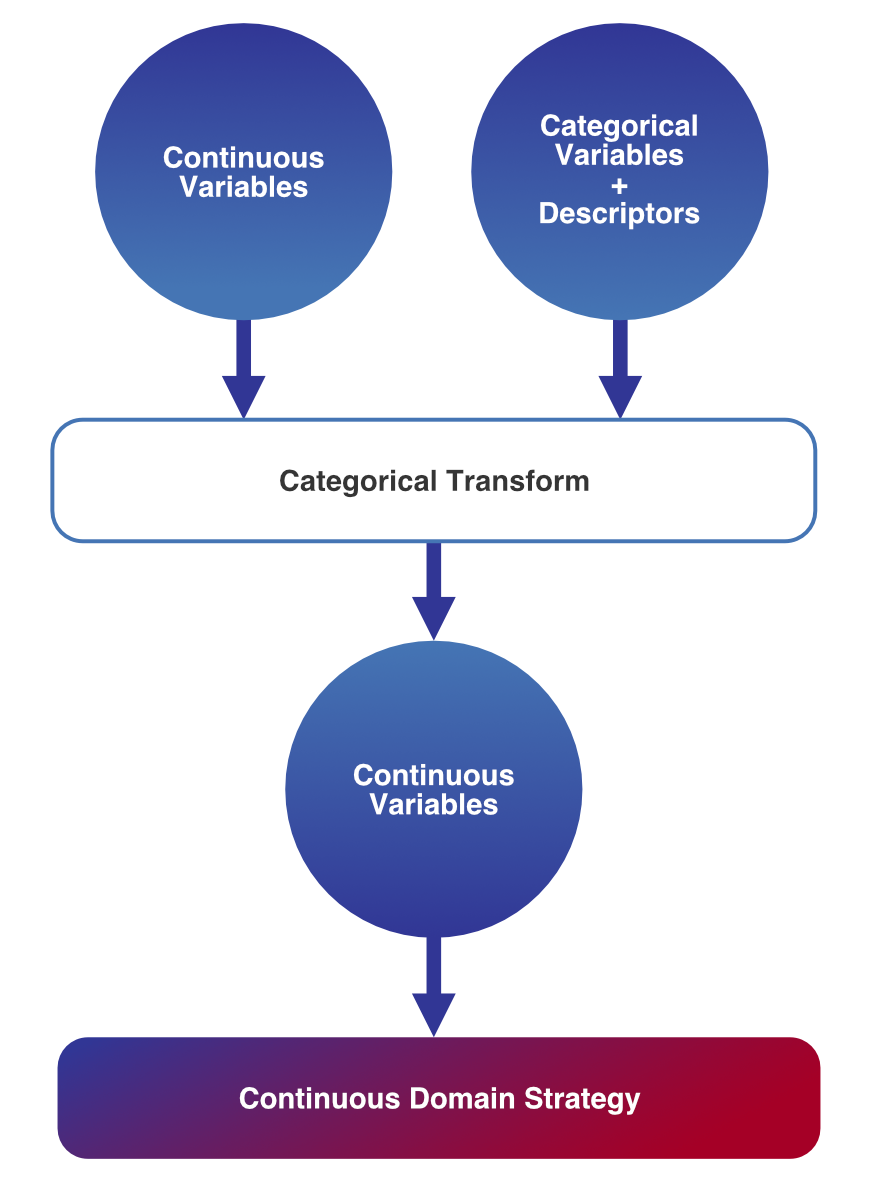
\includegraphics[width=0.5\linewidth]{gfx/Chapter03/categorical_transform.png}

    }
    \caption{(a) Schematic of achievement scalarisation functions which transform multi-objective optimisation problems into single objective problems. (b) Schematic of the categorical transform, which use descriptors to represent a categorical domain in continuous space.}
    \label{fig:transforms}
\end{figure}

Chimera is a hierarchical ASF developed by Hase et al. \cite{Hase2018b, Hase2020a}. Hierarchical means that the objectives are weighted, so the ASF will prioritise one objective over another. The main hyperparameters are the tolerances, which are values for each objective in $[0,1]$ that set how much each objective is weighted. A smaller tolerance indicates that the objective will be weighted more, while a larger tolerance indicates that the objective will be weighted less. The original paper does not give a clear mechanism for setting the tolerances, and the tolerances in the examples are tuned to the specific benchmarks used in the paper. To reflect what might be seen in practice, where the best optimal tolerances are not known in advance, we choose to round values for the tolerances and test four different combinations shown in Table \ref{tab:chimera_tolerances}. A smaller tolerance means that the objective will be weighted more, while a larger tolerance indicates that the objective will be weighted less. In this way, I aim to see if there was significant difference between different tolerance settings. In Figure \ref{fig:chimera_comparsion}, I show Chimera with different tolerances on the $S_NAr$ benchmark and experiment with the effect of these tolerances in the Results section.


\begin{table}
    \centering
    \caption{Tolerance combinations for Chimera used in benchmark tests.}
    \begin{tabular}{cc}
         Objective 1 & Objective 2  \\
         \hline
         0.5 & 0.5 \\
         0.5 & 1.0 \\
         1.0 & 0.5 \\
         1.0 & 1.0 \\
    \end{tabular}
    \label{tab:chimera_tolerances}
\end{table}

\begin{figure}
    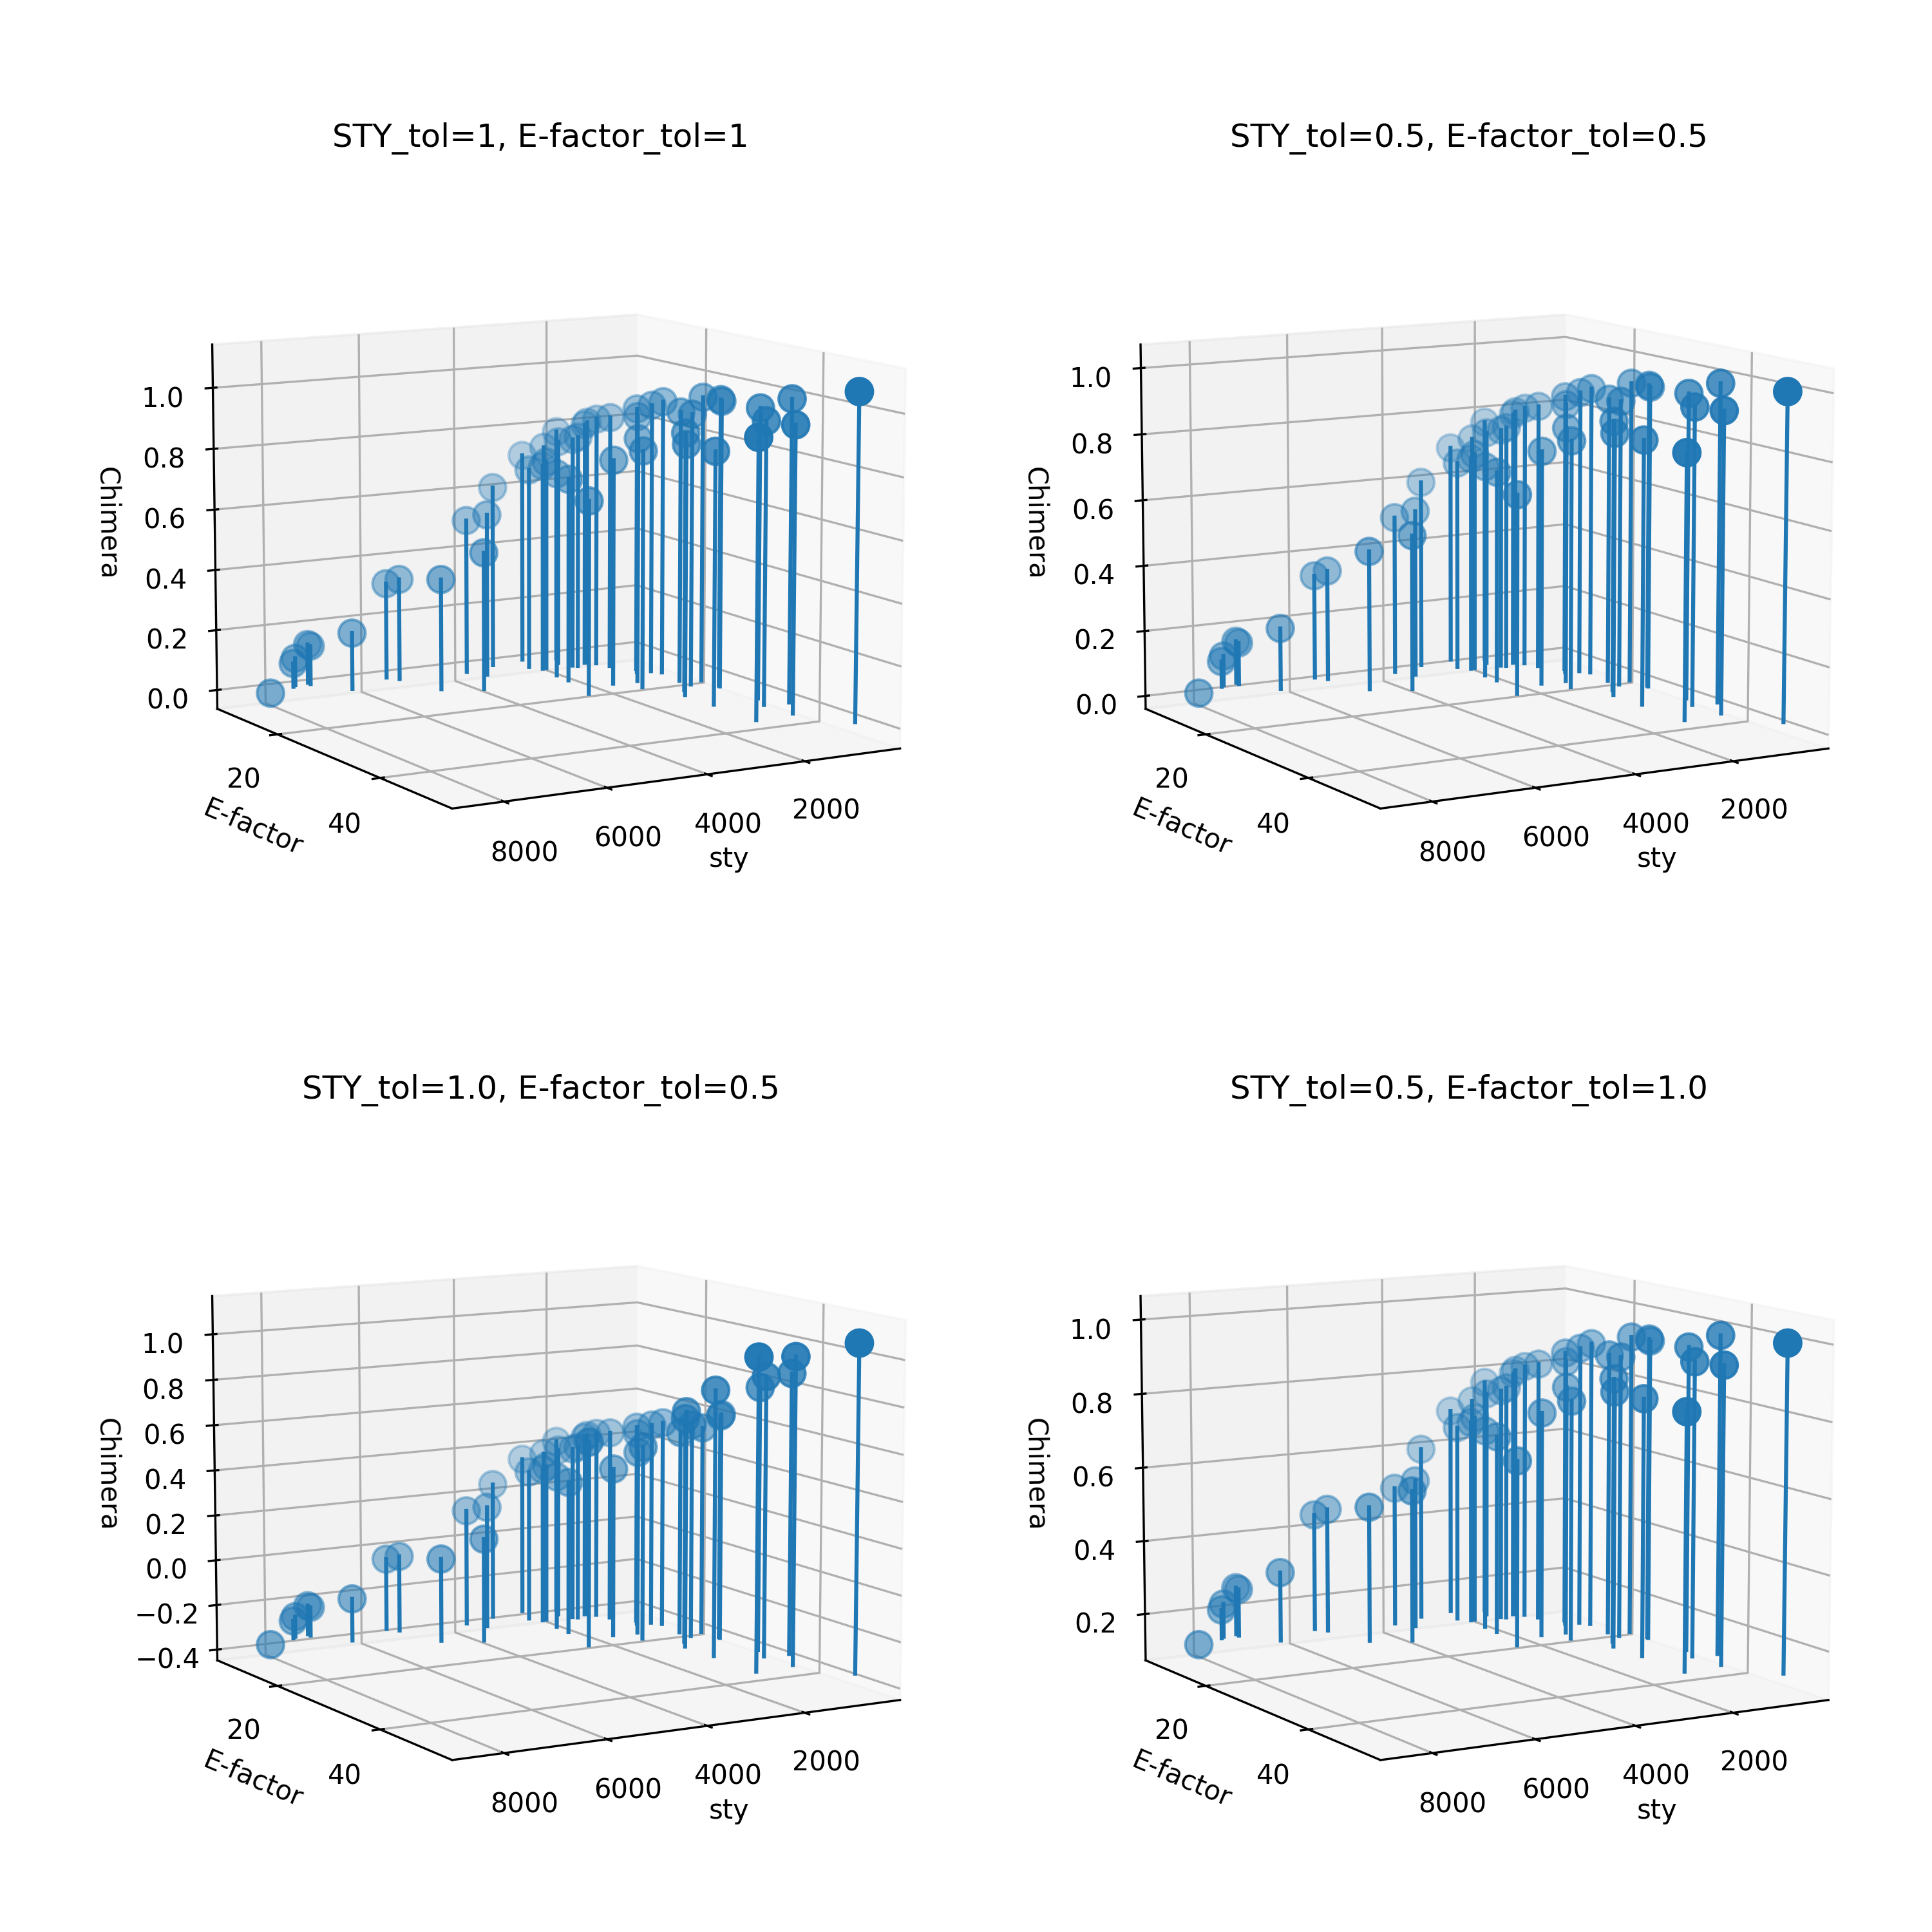
\includegraphics[width=\textwidth]{gfx/Chapter03/chimera_comparison.png}
    \caption{Comparison of the Chimera ASF on the SnAr Benchmark with different tolerances.}
    \label{fig:chimera_comparsion}
\end{figure}

\subsection{Computational Resources}
All tests run for the original Summit paper were completed on the University of Cambridge Service for Data-Driven Discovery (CSD3), with the exception of the NelderMead strategies. Each test was run on a single CPU with 32 threads. Example scripts for running the tests on a similar cluster or single servers are available on Github. 


\section{Results and Discussion}

\subsection{S\textsubscript{N}Ar optimisation highlights Bayesian strategies}
For the S\textsubscript{N}Ar benchmark, there is a negative correlation between STY and E-factor except for a very small Pareto front, so it is possible to optimize both simultaneously. As shown in Figure \ref{fig:S$_N$Ar_tsemo}a, as STY decreases, E-factor increases because increasing product throughput does not result in significantly greater environmental waste. Most of the waste comes from the flow of the solvent ethanol, which does not change significantly between reaction conditions \cite{Jeraal2020}. Only at very high space time yields is there a trade-off with E-factor due to decreased selectivity, and this part of the Pareto front (seen in Figure \ref{fig:snar}b) is not discovered by TSEMO.

\begin{figure}
    \centering
    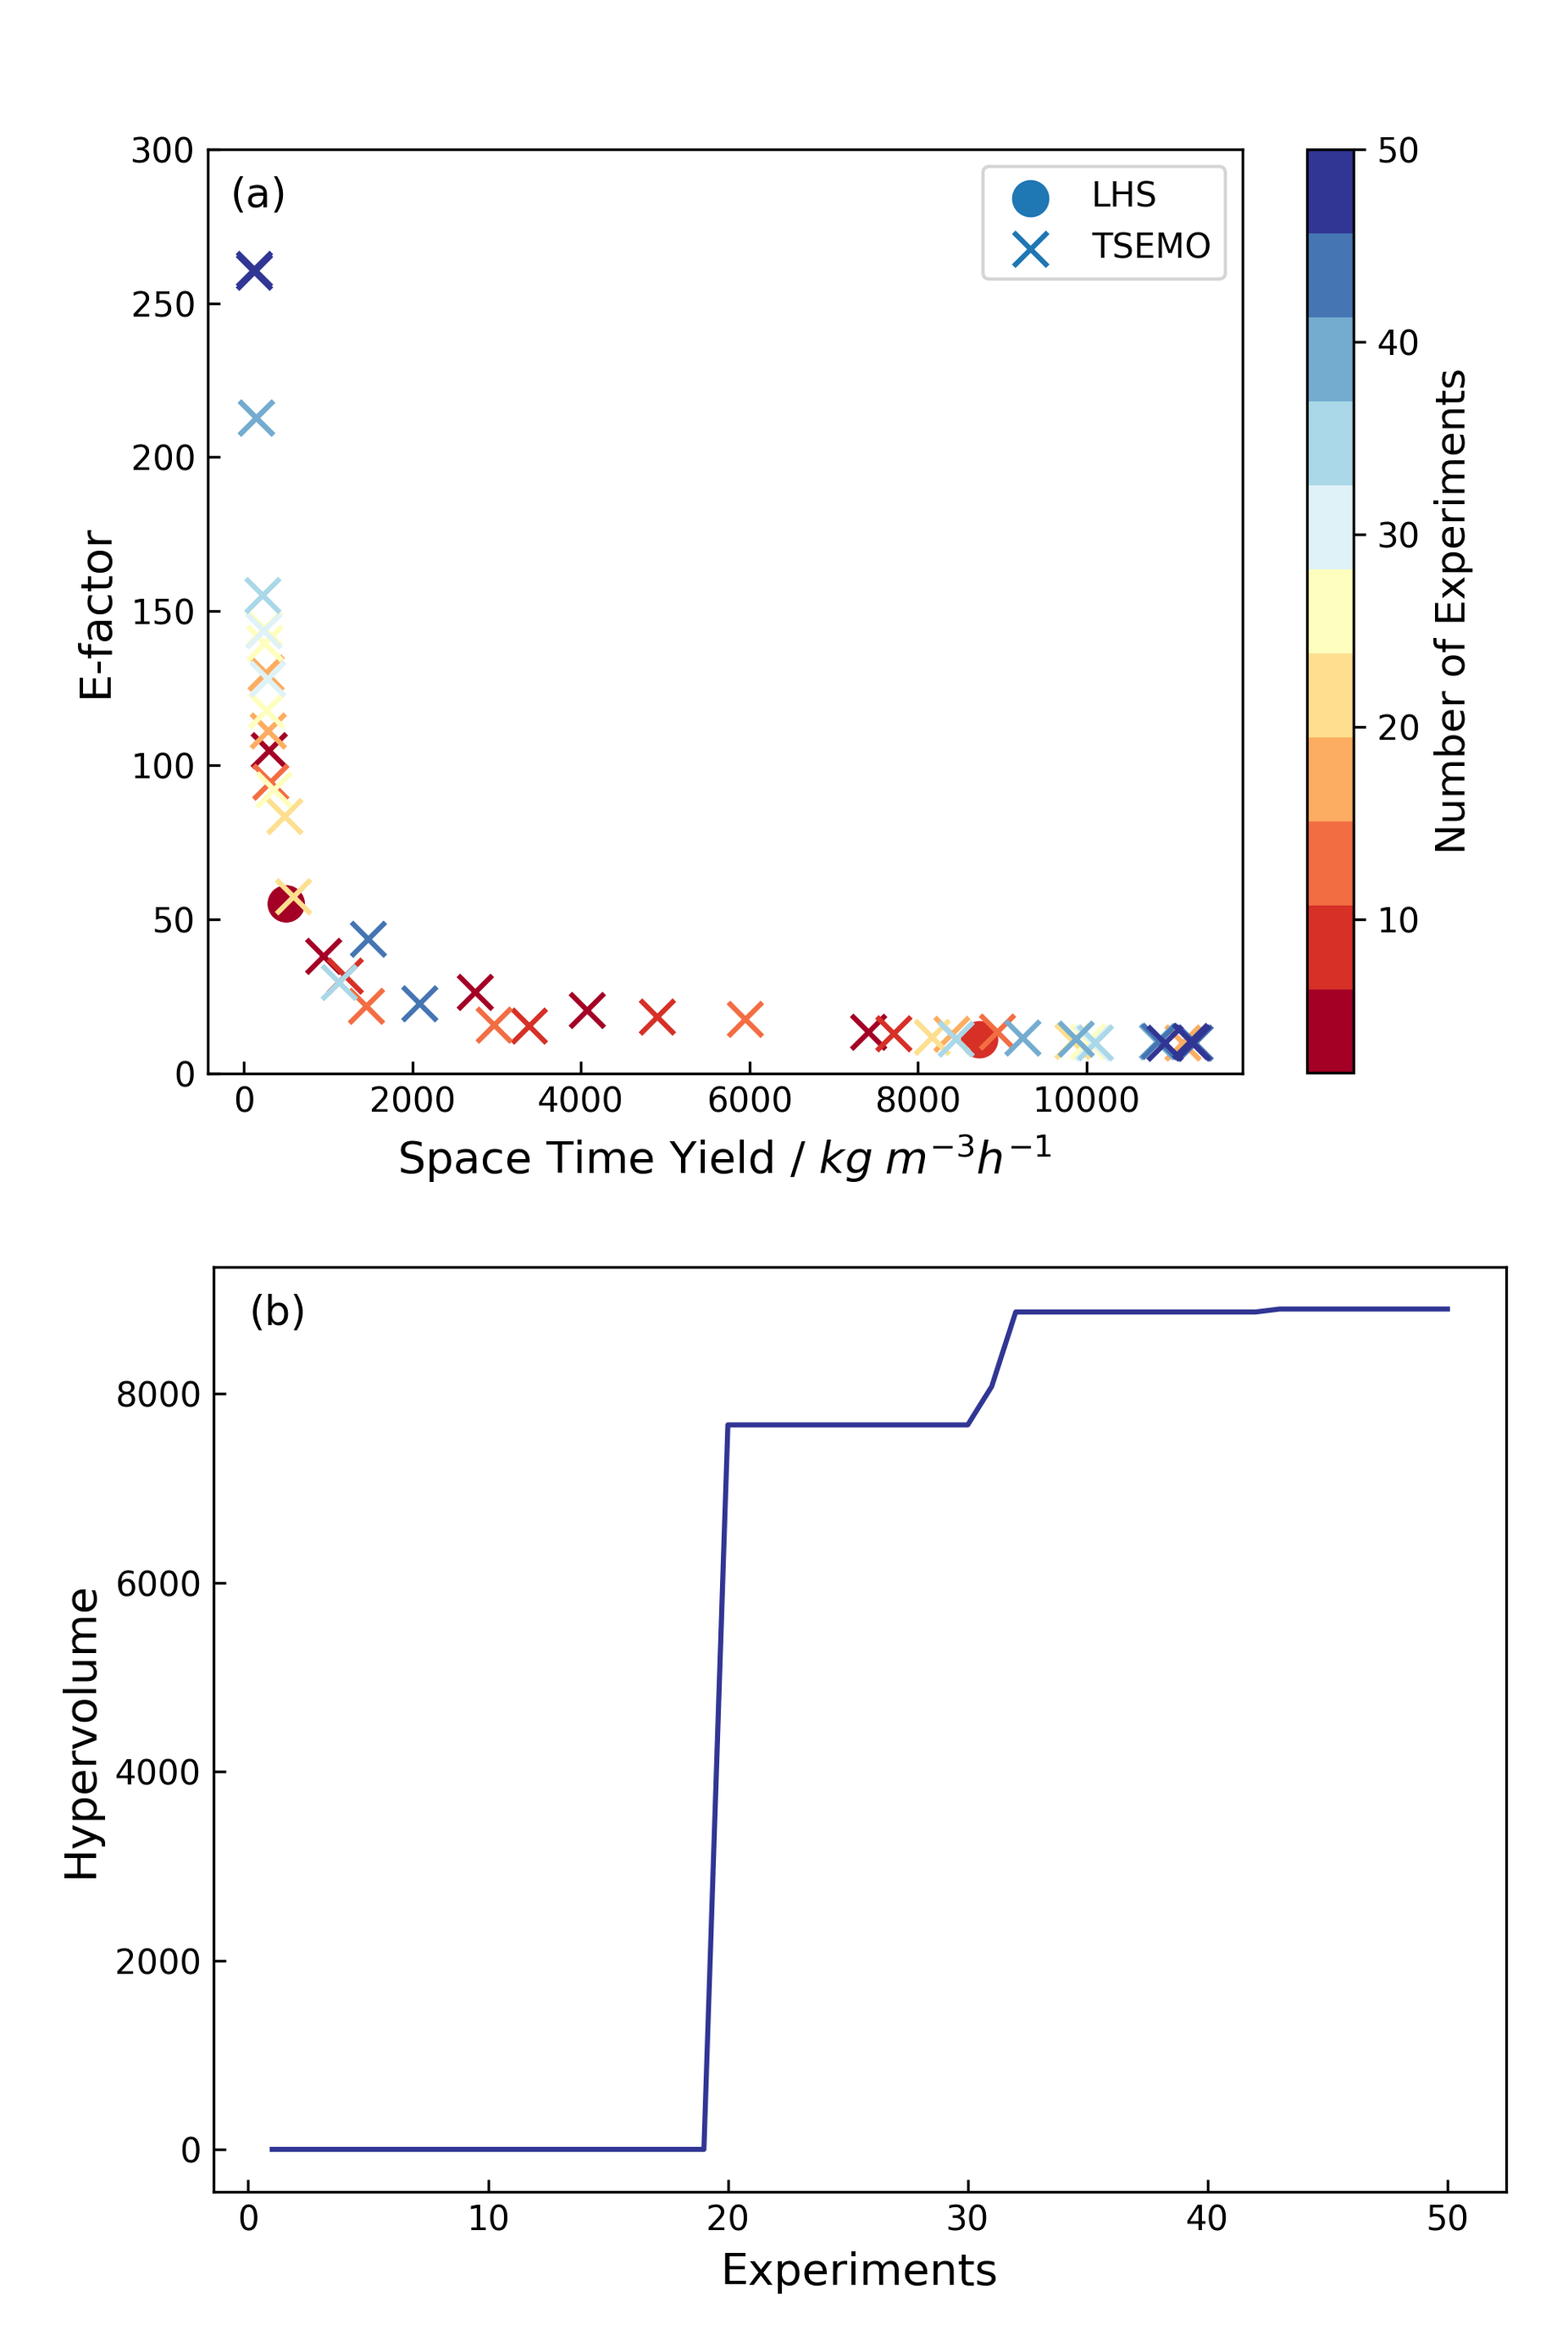
\includegraphics[width=0.65\textwidth]{gfx/Chapter03/snar_tsemo_pareto_hv.png}
    \caption{An exemplary optimisation of run of the S$_N$Ar benchmark with the TSEMO. (a) The objective values of each experiment suggested by TSEMO. TSEMO explores the parameter space and exploits to find conditions that give high space-time yield (>10,000 $(kg \; m^{-3} h^{-1}$) and low E-factor (<10.0). (b) Hypervolume trajectory of the optimisation run. Hypervolume is a measure of the number of optimal trade-offs between space-time-yield (STY) and E-factor found by a given machine learning strategy; larger hypervolumes correspond with more optimal solutions.}
    \label{fig:S$_N$Ar_tsemo}
\end{figure}

Out of the strategies implemented in Summit, only TSEMO is inherently able to handle multi-objective problems \cite{Bradford2018}. For the other strategies, I implement transforms that combine the objectives into a single value that can be optimised. Specifically, I implement Chimera (described previously) \cite{Hase2018b}, and I include a method for users to specify a custom transform of a multi-objective problem to a single objective problem \cite{Fitzpatrick2016, Epps2020}.

An exemplary run of TSEMO on the S$_N$Ar benchmark is shown in Figure \ref{fig:S$_N$Ar_tsemo}. Figure \ref{fig:S$_N$Ar_tsemo}a shows the objective values of each experiment suggested by TSEMO. The optimisation begins with two random experiments suggested by Latin Hypercube Sampling (LHS) \cite{McKay1979}, which are then followed by suggestions by TSEMO. Out of the first suggestions, only a few have optimal STY and E-factor values. With more data, TSEMO begins to select high concentrations of \textbf{1} (near 0.5 M), high equivalents of \textbf{2} (>3.5), and short residence times (30 seconds). However, a variety of temperatures give high STY and low E-factor. To illustrate the improvement with more experiments, I plot a measure of the quality of the pareto front called hypervolume. Since a larger hypervolume will always correspond with a better set of optimal values \cite{Zitzler2003}, I can see if the the optimisation strategy is finding conditions that result in better values for all objectives. As shown in Figure \ref{fig:S$_N$Ar_tsemo}b, the hypervolume starts at zero indicating no optimal points are found. Subsequently, hypervolume rapidly increases with more iterations, indicating better values of STY and E-factor are achieved.

Figure \ref{fig:hv_time_tradeoff} compares the performance of all strategies in Summit on the S$_N$Ar benchmark. Each strategy was run for a maximum of 50 iterations (i.e., 50 virtual reactions) and repeated with twenty different random starts to understand the influence of randomness on the performance of the strategy. Additionally, Chimera and the custom multi-objective transform were tested, and the best combination by terminal hypervolume for each strategy is shown. Figure \ref{fig:hv_time_tradeoff}a plots the hypervolume after 50 iterations and the average computation time per suggestion for each strategy. On average, the Bayesian optimisation strategies (GRYFFIN, SOBO, and TSEMO) perform best, finding the most optimal points in the allotted number of experiments. However, this performance comes at the price of three orders of magnitude greater computation cost. Furthermore, these tests were run on a high performance computing cluster with up to 32 threads dedicated for each strategy, and our experience is that the runtime increases by a factor of ten on consumer hardware.  The longer computation time is likely acceptable in the case of TSEMO given the improvement in performance since the time to suggest a new experiment might only add 5 to 10 \% in total time but give significant performance improvements. Interestingly, Nelder-Mead Simplex, which has been used in several studies \cite{McMullen2010b, Parrott2011, Sans2015, CortesBorda2016, Fitzpatrick2016, McMullen2010a, Poscharny2018}, failed to find any optimal points, even with ten random restarts on each run; in fact, random sampling performed better. This is because Nelder-Mead is a local search strategy, and I found that the multi-objective scalarisation functions (e.g., Chimera) have many local optima (see Figure \ref{fig:chimera_comparsion}). The DRO also failed to find optimal points, and SNOBFIT only had slightly better performance than random sampling.

\begin{figure}
    \centering
    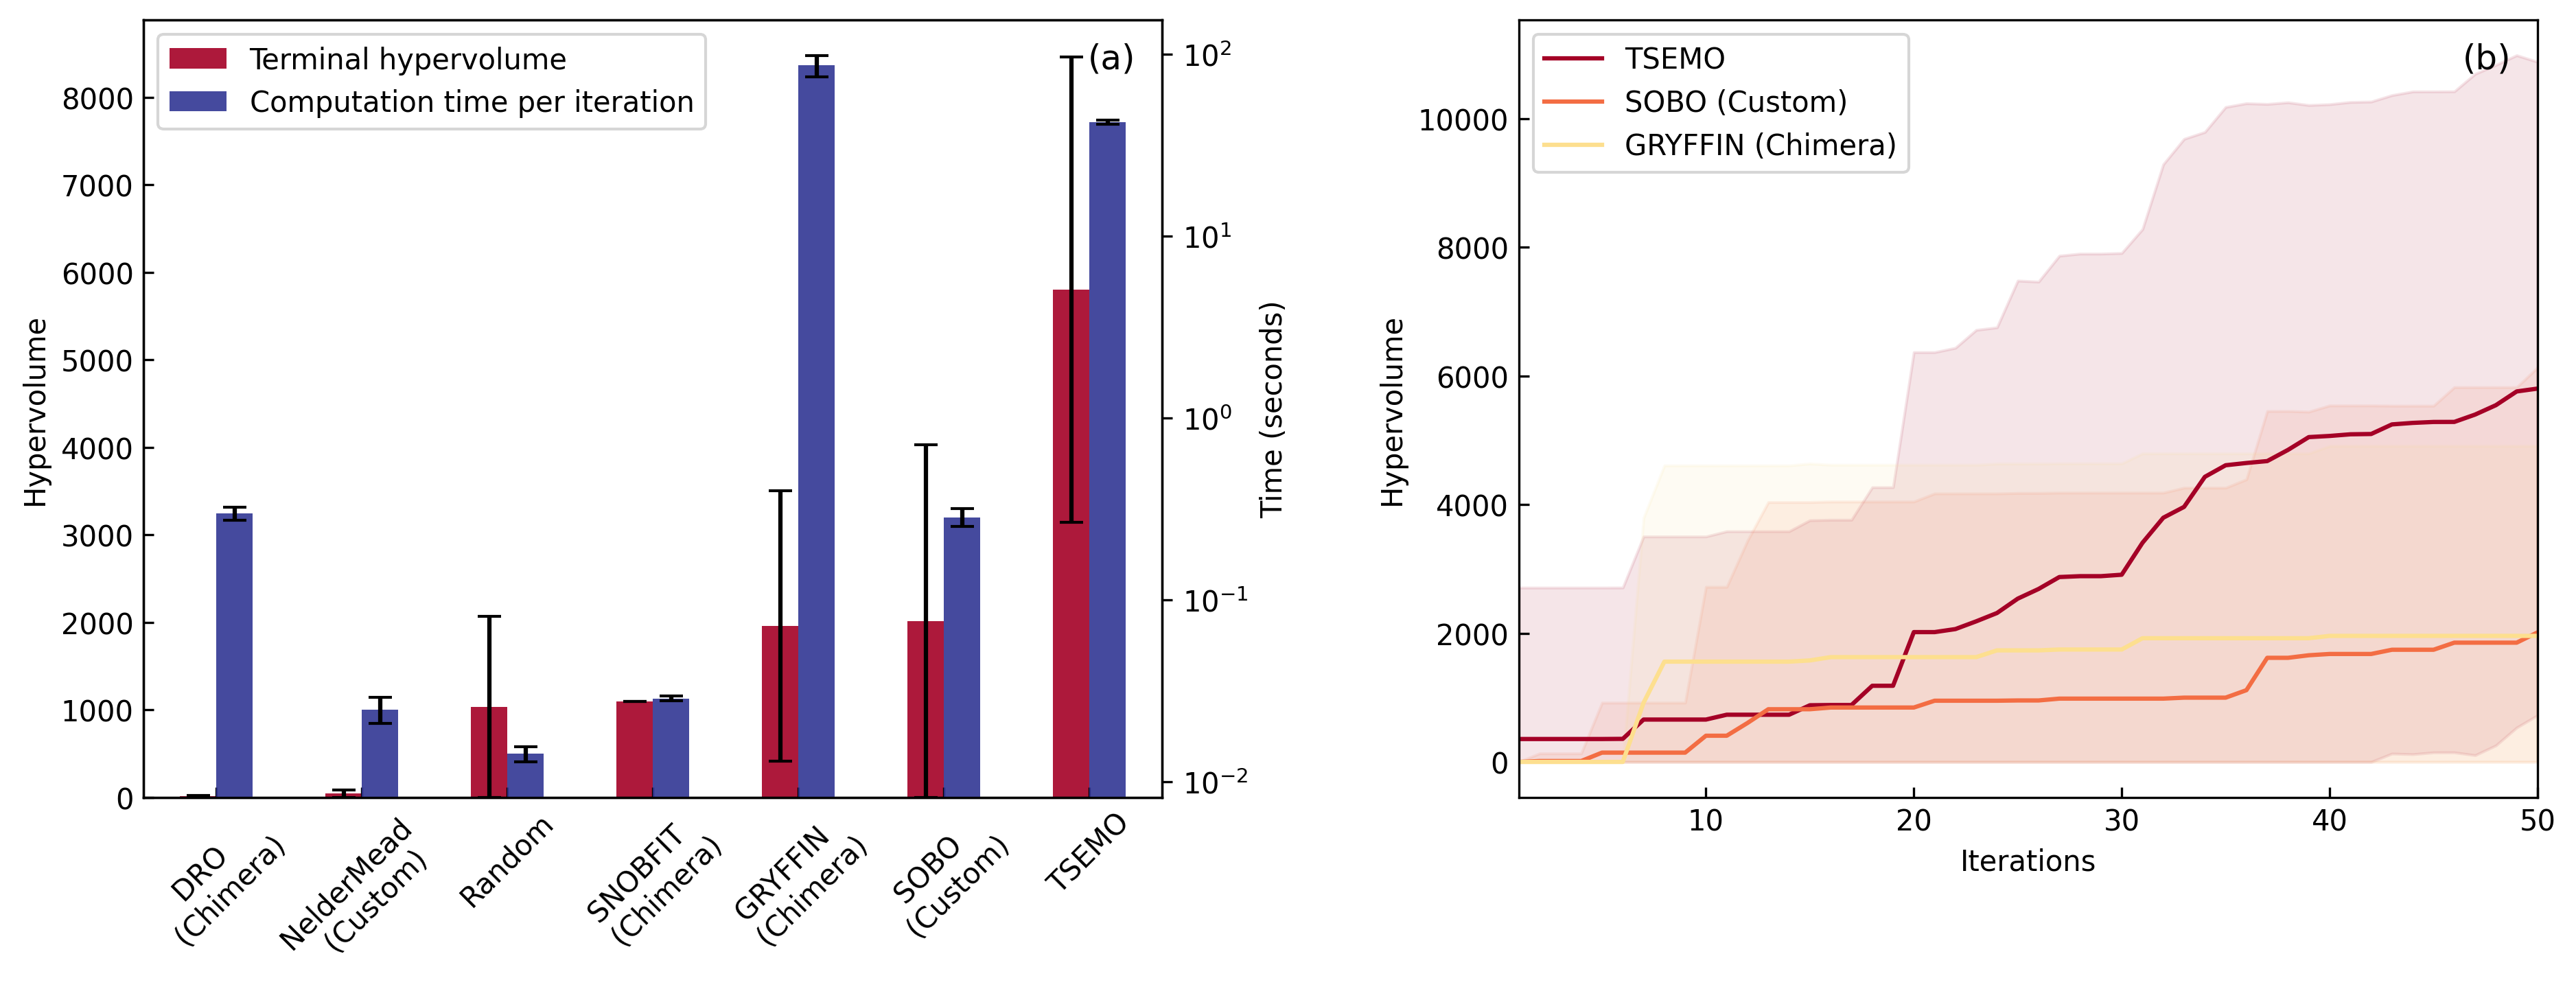
\includegraphics[width=0.75\textwidth]{gfx/Chapter03/snar_hv_time_tradeoff.png}
    \caption{Comparison of several strategies on the S$_N$Ar benchmark. (a) Trade-offs between improved performance and higher computation time. If used, a multi-objective transform is displayed in parenthesis. (b) Comparison of the hypervolume trajectories of three Bayesian optimisation strategies. The mean is plotted with the 95\% confidence interval.}
    \label{fig:hv_time_tradeoff}
\end{figure}

Figure \ref{fig:hv_time_tradeoff}b plots the average hypervolume of each of the Bayesian optimisation strategies over the course of 50 iterations. GRYFFIN quickly improves the quality of its suggestions with less than ten iterations, but TSEMO has better terminal performance. Both strategies have large confidence intervals with approximately 10 \% of repeats resulting in zero hypervolume. Still, their average performance is better than other strategies evaluated. The outstanding performance of TSEMO is likely linked to the fact that it trains individual surrogate models for each objective \cite{Bradford2018}, while the other strategies directly optimise the multi-objective transform value. As shown in Appendix \ref{ch:benchmarking_appendix}, there were not consistent patterns in which multi-objective transform worked best. Note that there is a large 95 \% CI in the hypervolume plots due to some optimisation runs failing to find the best catalyst.

\subsection{Optimisation of C-N Cross Coupling}

Strategies for the C-N cross coupling benchmark need to be able to select continuous variables (temperature, base equivalents, residence time) and categorical variables (the base and catalyst). Only SOBO and GRYFFIN can inherently work with categorical variables. To overcome this challenge, I calculated a set of descriptors or properties for the catalyst and base that transform the categorical variables into continuous variables. Previous work has shown that descriptors such as melting and boiling point or those from thermodynamic programs can help the optimisation \cite{Amar2019, Hase2020a}. I used the first two of five $\sigma$-moments from computational fluid thermodynamics program COSMO-RS as these act as universal descriptors for any molecule \cite{Zissimos2002}. I would prefer to use all five $\sigma$-moments, but I found that it is difficult to optimise in the resulting fourteen-dimensional input space. Using only the first two $\sigma$-moments for the catalyst and base makes it a seven-dimensional input space (three continuous variables and two categorical variables with two descriptors each).  Note that DRO is not included because my collaborator Jan Rittig empirically found that pre-training the policy on input spaces greater than six-dimensions was very slow. Since the C-N benchmark was also a multi-objective problem, I used the same transforms as in S$_N$Ar benchmark.

\begin{figure}
    \centering
    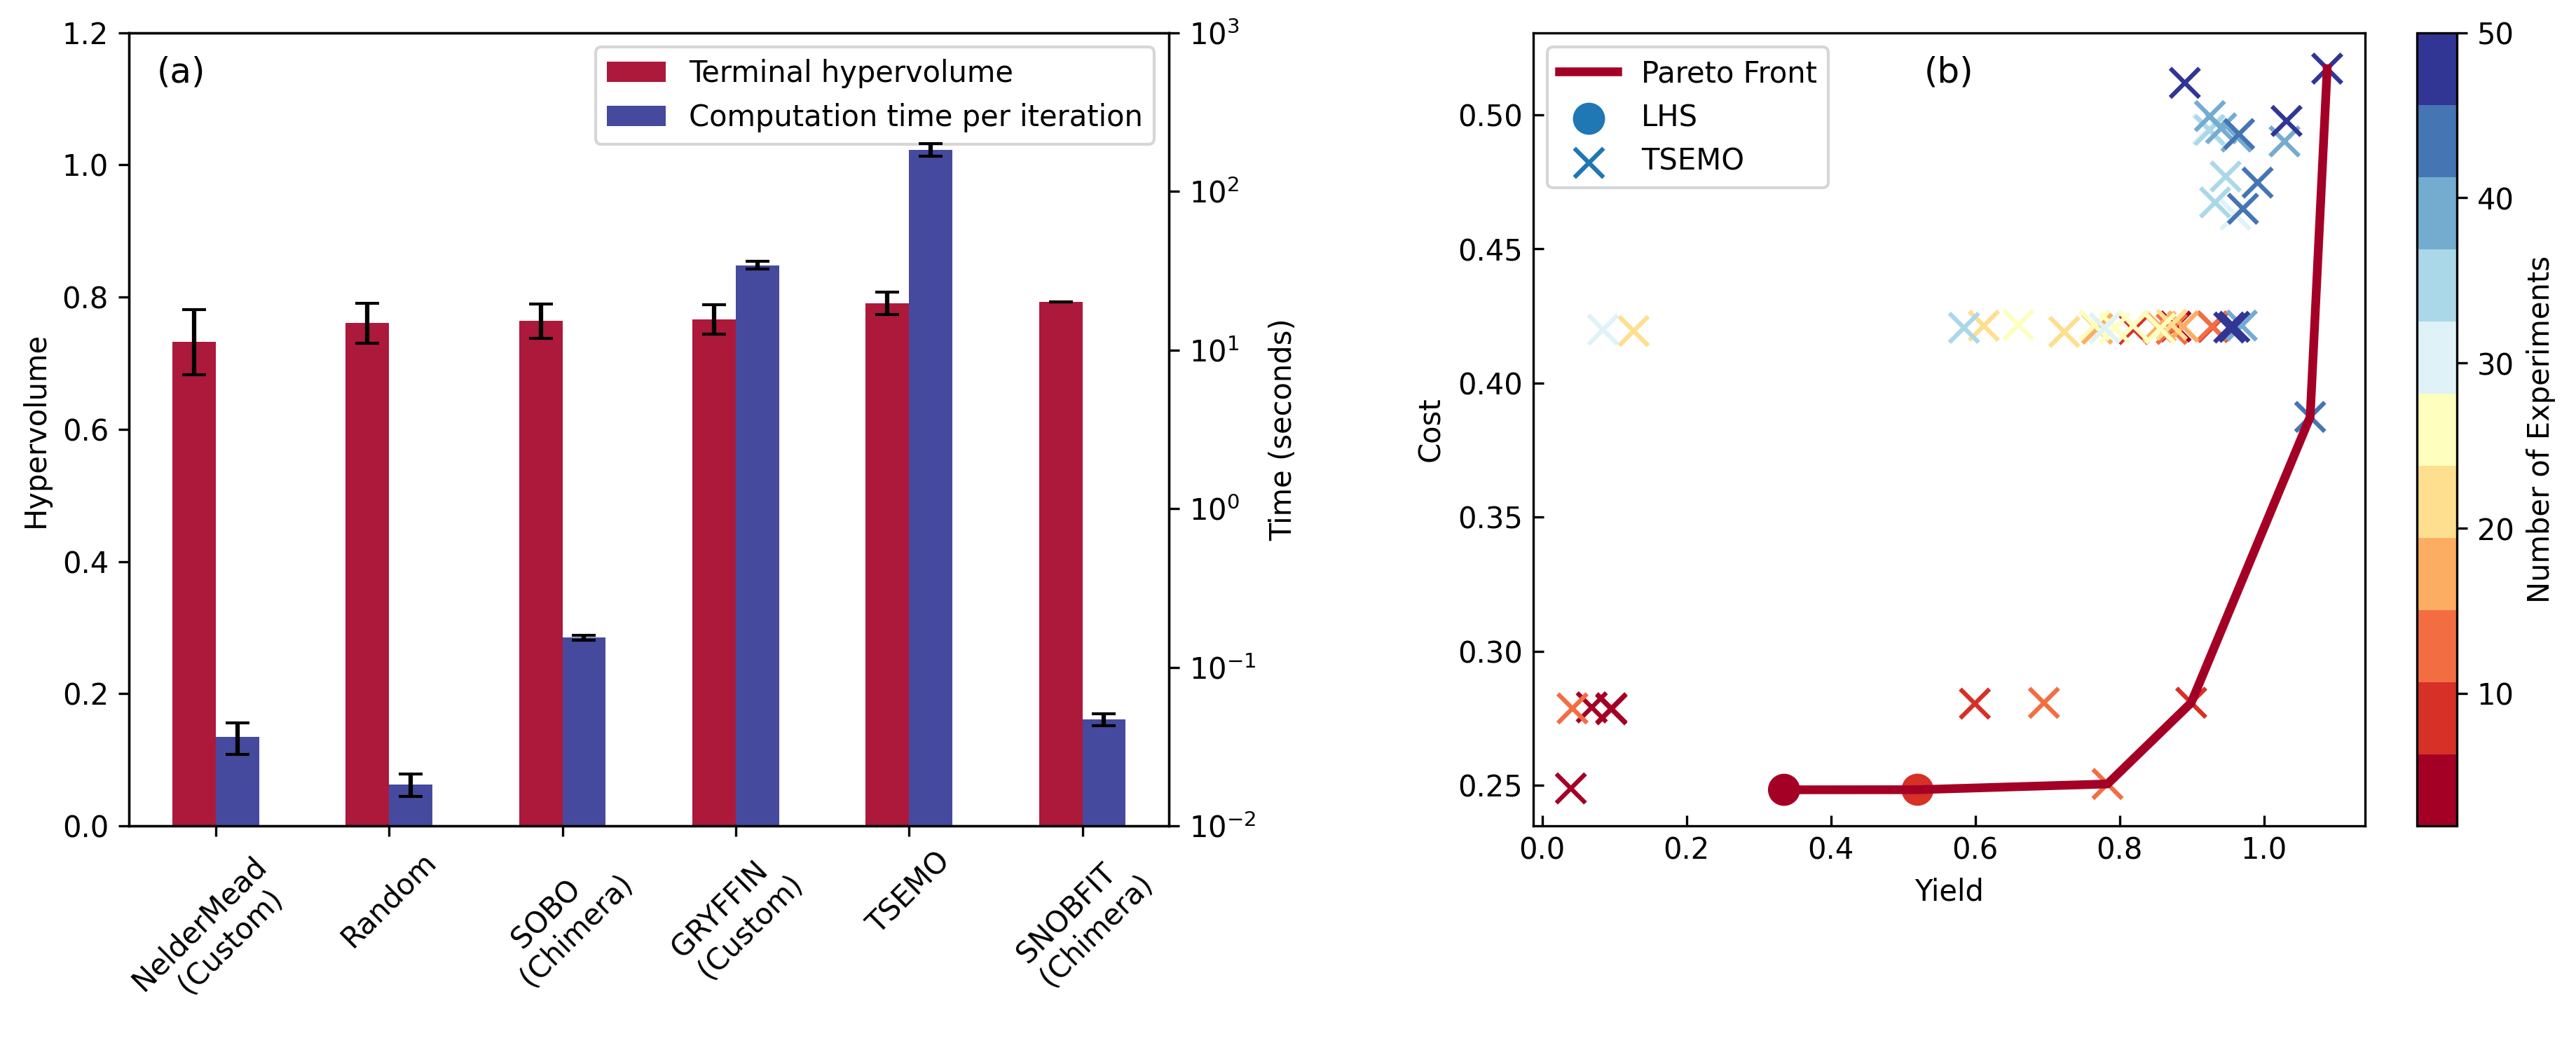
\includegraphics[width=0.7\textwidth]{gfx/Chapter03/cn_hv_time_tradeoff.png}
    \caption{Comparison of several strategies on the C-N benchmark. (a) Performance of various optimisation strategies. If used, a multi-objective transform is displayed in parenthesis. (b) Comparison of the hypervolume trajectories of top performing strategies. The mean is plotted with the 95\% confidence interval.}
    \label{fig:cn_hv_time}
\end{figure}

As shown in Figure \ref{fig:cn_hv_time}a, the performance across strategies is very similar for this benchmark, almost indistinguishable. For example, the results of the random selections are nearly equivalent to the machine learning strategies. I suggest this is because the effective parameter space is quite small. Once the optimal catalyst and base are selected, only three variables need to be tuned (reaction temperature, residence time and base equivalents). Furthermore, I see no noticeable difference between the strategies that use descriptors and those that do not use descriptors (SOBO and GRIFFYN).

The C-N benchmark presents trade-offs in the objectives. Increasing yield often results in an increase in cost. This series of optimal trade-offs between yield and cost is called a Pareto front. In Figure \ref{fig:cn_hv_time}b, I plot the objective values for one optimisation of C-N benchmark using TSEMO. With more experiments, the Pareto front is better filled out and a greater proportion of selections have high yield. As shown in Table \ref{tab:cn_benchmark_results}, the optimal catalyst complex is AlPhos, in line with results from Baumgartner et al \cite{Baumgartner2019}. However, it is clear that some conditions result in a prediction of yield being greater than 100 \%. Some of the original data has yield greater than 100 \%, apparently due to small errors in HPLC measurements \cite{Baumgartner2019}. Since the data-driven model has no concept of chemistry (i.e., that yield cannot be greater than 100 \%), it simply learns this pattern and extrapolates it. However, this lack of physical constraints is not a significant issue because the model simply needs to learn to order the conditions correctly from lowest to highest yield in order to guide the optimisation.

\begin{table}[tb]
    \centering
    \caption{Pareto front data from one run of the C-N Benchmark using TSEMO. See the SI for more information about the C-N benchmark, including the catalysts and bases used.
    }
    \begin{tabular}{llrrrrr}
    \hline
         \textbf{Catalyst} &  \textbf{Base} & \textbf{Base Equiv} & \textbf{Temp ($^{\circ}$ C)} &       $\boldsymbol{\tau}  (s)$ &     \textbf{Yield} &      \textbf{Cost (\$)} \\
    \hline
     tBuXPhos &   TMG &             1.32 &       89.86 &   117.73 &  34 \% &  0.25 \\
     tBuXPhos &   TMG &             2.38 &       64.35 &  1594.63 &  52 \% &  0.25 \\
     tBuXPhos &   DBU &             2.03 &       71.12 &  1040.59 &  78 \% &  0.25 \\
 tBuBrettPhos &   DBU &             2.28 &       87.16 &   107.66 &  90 \% &  0.28 \\
 tBuBrettPhos &  BTMG &             2.50 &       99.32 &  1081.24 &  100 \% &  0.39 \\
       AlPhos &  BTMG &             2.25 &       99.89 &  1763.66 &  100 \% &  0.52 \\
    \end{tabular}

    \label{tab:cn_benchmark_results}
\end{table}

\section{Conclusions}

Summit is a framework for optimisation of chemical reactions. I present two benchmarks for reaction optimisation and compare the performance of seven strategies with various combinations of multi-objective transforms on these benchmarks. Our results show that Bayesian optimisation performs most consistently with TSEMO showing best-in-class performance on both benchmarks.

Summit enables researchers to test new optimisation strategies without expensive experiments. I envision that new benchmarks could address outstanding challenges in reaction optimisation such as multi-step optimisation \cite{Coley2019, Clayton2020} and mixed objective domains (i.e., categorical and continuous objectives). Additionally, I foresee that new strategies can be tested against current and future benchmarks for performance assessment. Summit provides a simple method for implementing new benchmarks either as mechanistic models or by training data-driven models based on past experiments.

Furthermore, since we released Summit, the major use case has been optimisation of flow chemistry processes. For example, van der Westhuizen et al used Summit to build an automated flow chemistry platform and optimized an allylation of isovanillin \cite{Van2022}. Similarly, in unpublished work from the Lapkin lab, Summit has been used to optimize a Suzuki coupling reaction in an automated flow chemistry reactor. This supports the concept described in Chapter \ref{ch:introduction} of using optimisation to assist in development of new processes.

In the optimisation community, the idea of "No-free lunch" is often cited \cite{Wolpert1997}. The principle is that an optimisation strategy that works well for one problem will inherently be bad for another.  This implies that understanding the strengths and weaknesses of each optimisation strategy are important. Here, I have identified that Bayesian optimisation is an efficient way to overcome the challenges of reaction optimisation. In the following chapter, I build on this insight to improve Bayesian optimisation using transfer learning.
